

\begin{table*}
  %\vspace{-0.2in}
  \centering
\begin{threeparttable}
  \caption{Implementations and Parameter Settings of the Considered Baselines}\label{table:baselines}
\begin{tabular}{llclc}\toprule
  \multicolumn{1}{c}{\textbf{Algorithm}}          &
  \multicolumn{1}{c}{\textbf{Classification}}     &
  \multicolumn{1}{c}{\textbf{Implementation}}     &
  \multicolumn{1}{c}{\textbf{Parameter Settings}} &
  \multicolumn{1}{c}{\textbf{Reference}} \\\midrule
  OSRAD  & Diffusion       & Custom            & \(W_{\text{kuan}}= 5 \times 5\), \(c_{\text{tang}} = 0.1\), \(N_{\text{iteration}}=30\), \(\Delta t = 1\) & \cite{krissian_oriented_2007}  \\
  ADMSS  & Diffusion       & Official\tnote{1} & \(N_{\text{class}} = 4\), \(N_{\text{memory}}=5\), \(N_{\text{iteration}} = 20\), \(\sigma = 0.1\), \(\rho = 0.1\)  & \cite{ramos-llorden_anisotropic_2015} \\
  LPNDSF & Diffusion       & Custom            & \(r = [0.1, 1.0, 0.1]\), \(k = [0.3, 0.1, 0.1]\) & \cite{zhang_multiscale_2006} \\
  MNLM   & Non-local mean  & Custom            & \(M = 19 \times 19\), \(K = 3 \times 3\), \(I = 5\), \(h=0.1\) & \cite{breivik_realtime_2017} \\
  NLLR   & Non-local mean \& Low-rank recon.   & Official\tnote{2} & \(H = 10\), \(\beta = 10\) & \cite{zhu_nonlocal_2017} \\
  PFDTV  & Diffusion \& TV regularization    & Custom\tnote{3}   & \(N_{\text{iteration}} = 10\), \(s=15\) & \cite{mei_phase_2020} \\
  \bottomrule
\end{tabular}
\begin{tablenotes}
  \item[1] \url{https://www.mathworks.com/matlabcentral/fileexchange/52988-anisotropic-diffusion-with-memory-based-on-speckle-statistics-for-ultrasound-images}
  \item[2] \url{https://appsrv.cse.cuhk.edu.hk/~lzhu/webpage_despeckling_cvpr2017/index.html}
  \item[3] Based on the official implementation available at \url{https://github.com/Binjie-Qin/PFDTV}.
\end{tablenotes}
\end{threeparttable}
\vspace{-0.1in}
\end{table*}

%%% Local Variables:
%%% TeX-master: "master"
%%% End:

%

\section{Experiments}\label{section:eval}

\subsection{Experimental Setup}
We now use the Ultrasound Design Gallery for tuning the cascaded Laplacian pyramid diffusion.

\subsubsection{Experiment Design}
%\paragraph{Sonographer Subjects}
We recruited five sonographers and a cardiologist from the Kangbuk Samsung Hospital Total Healthcare Center (Seoul, South Korea, Republic of) and asked them to optimize a video sequence of a liver images and two sequences of echocardiographic heart images.
All five sonographers are Registered Diagnostic Cardiac Sonographers (RDCS) certified by the American Registry for Diagnostic Medical Sonography (ARDMS) with at least three years of practicing experience.
The cardiologist is actively practicing and has ten years of clinical experience.
For convenience, the expert subjects are alphabetically coded from A to F where A is the cardiologist.

\begin{table}
  \centering
  \caption{Hardware used for the Experiments}\label{table:specs}
  \begin{threeparttable}
  \begin{tabular}{ll}
    \toprule
    \multicolumn{1}{c}{\textbf{Type}}
    & \multicolumn{1}{c}{\textbf{Model and Specifications}}
    \\ \midrule
    Processor & Intel i7--7700HQ, 2.8 GHz (maximum 3.8 GHz) \\
    GPU       & Nvidia GeForce GTX 1050 Mobile \\
    Display   & Sharp LQ156D1, 15.6 inch, \(3840 \times 2160\), 282ppi  \\
    Memory    & 16GB DDR4--2400 \\ \bottomrule
  \end{tabular}
  \end{threeparttable}
\end{table}
%
%\paragraph{Experiment Protocol}
Each of the sonographers were given access to the~\usdg~through same laptop.
The hardware specification of the laptop are shown in~\cref{table:specs}.
Then, the sonographers interact with the~\usdg~until the iteration counter indicated 15.
The first 4 iterations used random settings such that \(\vx\) is a random uniform vector and \(\vxi\) is sampled from a unit \(L_{\infty}\) hypersphere.

The sonographers were instructed to freely interact with the video control panel at any time.
However, they were strictly instructed to choose a position on the slider \textit{relative} to other positions.
Without such instruction, some users were unable to choose a candidate becase all of the positions seemed to result in equality disliked images.
Also, in some cases, all of the positions on the slider resulted in images visually indistinguisable.
For such iteration, We instructed the sonographers to choose a random position.

For evaluating the final results, we choose the parameter setting maximizing the mean utility function of each sonographer such as \( \vx^* = \argmax_{\vx} \mu\left(\vx \mid \mathcal{D}_{15} \right) \).
The cascaded Laplacian pyramid setting acquired from each expert subject is denoted as CLPD-\texttt{[code]} where the trailing letter \texttt{[code]} is the subject code.

\subsubsection{Ultrasound Image Data}
We use three \textit{in vivo} ultrasound image sequences.
A liver subcostal view sequence, a echocardiac 4-chamber view sequence, and a echocardiac parasternal long-axis view sequence.
The liver sequence was a acquired at Sogang University (Seoul, South Korea, Republic of) from a volunteer using a Samsung Accuvix V10 scanner and a Samsung C2--5EL convex probe, while the echococardiac parasternal long-axis sequence was acquired using a GE Vivid E90 scanner with a probe.
The echocardiac 4-chamber view sequence was extracted from the CAMUS challenge dataset~\cite{leclerc_deep_2019}, which was acquired using a GE Vivid E95 scanner with a GE M5S probe.

Since the Samsung Accuvix V10 scanner research package returns beamformed radio-frequency (RF) data, we performed DC rejection, envelope detection, and then scan conversion locally.
The RF data has 128 scanlines, which we lateral interpolate by a factor of 8.
A prealias filter was used before scan conversion.
For the GE Vivid E90 scanner, we extracted the quantized images from the raw DICOM files, and performed scan conversion.

\subsubsection{Image Enhancement Baselines}
We evaluate the tuned cascaded Laplacian pyramid diffusion filters against a diverse range of speckle reduction algorithms.
Among diffusion algorithms, we compare against the speckle reducing anisotropic diffusion (OSRAD,~\cite{krissian_oriented_2007}), the anisotropic diffusion filter with memory based on speckle statistics (ADMSS,~\cite{ramos-llorden_anisotropic_2015}), and the multiscale nonlinear diffusion and shock filter (LPNDSF,~\cite{zhang_multiscale_2006}) methods.
Among non-local means based methods, we compare against the multiscale non-local means (MNLM,~\cite{breivik_realtime_2017}), and the non-local low-rank patch recovery (NLLR,~\cite{zhu_nonlocal_2017}) methods.
Lastly, we compare against the phase asymmetry ultrasound despeckling with fractional anisotropic diffusion and total variation (PFDTV,~\cite{mei_phase_2020}) method.

\subsubsection{Implementations and Tuning of the Baselines}
To ensure a fair comparison, we will use the official implementation of the considered baselines whenever available.
The implementations and parameter settings of the considered baselines are organized in~\cref{table:baselines}.
For the OSRAD, MNLM, LPNDSF, and PFDTV algorithms, we reimplemented the algorithms according to the descriptions in the original papers.
While the official implementation of PFDTV is publically available online, we had to reimplement it due to numerical issues.

%\paragraph{Issues with Pixel Spacing}
For the NLLR and PFDTV, the pixel spacing of the data used in the original works (\(300 \times 225\)) differed significantly with ours (our images are \(800 \times 600\)).
Because of this, when applied to our data, the results were qualitatively different from those reported in the original papers.
Thus, for PFDTV and NLLR, we downscaled the images by \(40\%\), applyed the respective methods, and then upscaled the images for evaluation.

%\paragraph{Input Transformations}
While often not clearly stated, the input format of ultrasound speckle reduction methods vary.
For example, OSRAD requires the input image to be in natural scale rather than logarithmic scale.
Therefore, for OSRAD, we decompressed the log-compressed images as recommended by~\cite{yongjianyu_generalized_2004} and then recompressed the output.
Other than OSRAD, we applied all methods to log-compressed images with pixel intensities in the range of \([0, 255]\).

\subsubsection{Metrics}
For objective quality assessment, we apply the following quality metrics to the image \textit{before} dynamic range adjustment.
All results are presented up to three significant digits.

\paragraph{(Speckle) Signal-to-Noise Ratio (SNR)}
The SNR measures the amount of speckle noise relative to the mean response of a region-of-interest.
It is given as
\begin{align}
  \mathrm{SSNR} \texttt{[dB]} = 10 \log_{10} \frac{\mu}{\sigma}
\end{align}
where \(\mu\) is the mean response and \(\sigma\) is the standard deiviation of the region-of-interest.
When computed against a fully-formed speckle region, the SNR is called the \textit{speckle} SNR (SSNR).
In this case, \(\sigma\) corresponds to the noise standard deiviation.
We present the SNR in decibel scale.

\paragraph{Contrast-to-Noise Ratio (CNR)}
The CNR first introduced by Patterson and Foster~\cite{patterson_improvement_1983} measures the mean response difference of two regions-of-interests relative to their standard deviations such as
\begin{align}
  \mathrm{CNR} \texttt{[dB]} = 10 \log_{10} \frac{| \mu_{1} - \mu_{2} |}{ \sqrt{\sigma^2_1 + \sigma^2_2} }
\end{align}
where \(\mu_1, \mu_2\) are the mean responses of the regions-of-interests, and \(\sigma_1, \sigma_2\) are their standard deviations, respectively.
While the CNR is loosely related to the lesions detectibility~\cite{smith_ultrasound_1984}, Rindal \textit{et al.} has shown that it is less reliable across dyfferent dynamic ranges~\cite{rindal_effect_2019}.
We present the CNR in decibel scale.

%% Nonetheless, the CNR still provides a measure of relative contrast.

\paragraph{Generalized CNR (gCNR)}
As a remedy to the limitations of the CNR, Rodriguez-Molares \textit{et al.}~\cite{rodriguez-molares_generalized_2020} proposed the gCNR metric.
They also showed that it is less affected by dynamic range alternations, making it a better general performance metric.
The gCNR is defined as
\begin{align}
  \text{gCNR} = 1 - \int_{-\infty}^{\infty} \min\big(p_1\left(x\right), p_2\left(x\right)\big) \, dx
\end{align}
where \(p_1\left(x\right)\) and \(p_2\left(x\right)\) are the probability densities of \(x\) subject to the pixel intensity distributions of the regions-of-interests 1 and 2.

\paragraph{Structural Similarity Index (SSIM)}
The SSIM is a metric for measuring the \textit{structural} similarity of images, which is derived as a product of the differences in lumiance, structure, and contrast~\cite{wang_image_2004a}.
Wang \textit{et al.} has shown that the SSIM is aligned with the perception of humans, and is sensitive to distortions such as blur and blockiness.
Mathematically, the SSIM between image 1 and 2 is computed such that
\begin{align}
  \mathrm{SSIM} = \frac{1}{N} \sum_k^N \frac{
    (2 \mu_{1,k} \, \mu_{2, k} + C_1)(2 \sigma_{12, k} + C_2)
  }{
    (\mu_{1,k}^2 + \mu_{2,k}^2 + C_1) ( \sigma_{1,k}^2 + \sigma_{2,k}^2 + C_2)
  }
\end{align}
where \(\mu_{1,k}\), \(\mu_{2,k}\), are the mean of the \(k\)th patch on each images, \(\sigma_{1,k}^2\), \(\sigma_{2,k}^2\) are their respective variances, and \(\sigma_{12, k}\) is the covariance of the two.
The SSIM is taken as an average over all the patches, which are taken by a \(11 \times 11\) Gaussian window of standard deviation 1.5.
The coefficients are chosen as \(C_1 = 1 \times 10^{-4}, C_2 = 9 \times 10^{-4} \).
We use the implementation of the \texttt{ImageQualityIndexes.jl} library\footnote{\url{https://github.com/JuliaImages/ImageQualityIndexes.jl}}

\paragraph{\(S_3\) Index}
Finally, we use a metric for evaluating the blurriness of the images.
Blurriness metrics have not been tradiionally used for evaluating the quality of medical ultrasound images.
However, we will later show that blurriness is an important quality factor for sonographers.
In this work, we use the \(S_3\) metric proposed in~\cite{vu_bf_2012}.
The \(S_3\) value of the \(k\)th patch is defined as a harmonic mean such that
\begin{align}
  S_3\left(k\right) = \sqrt{S_1\left(k\right)} \sqrt{S_2\left(k\right)}
\end{align}
where \(S_1\left(k\right)\) and \(S_2\left(k\right)\) are its spatial and spectral measures of sharpness.
The final \(S_3\) index of an image is given as the average of the top 1\% \(S_3\) values.
We use the official implementation\footnote{\url{https://sites.google.com/site/cuongvt101/research/Sharpness-measure}} provided by the authors.

%
\begin{figure}[h]
  \centering
  \subfloat[Liver image]{
    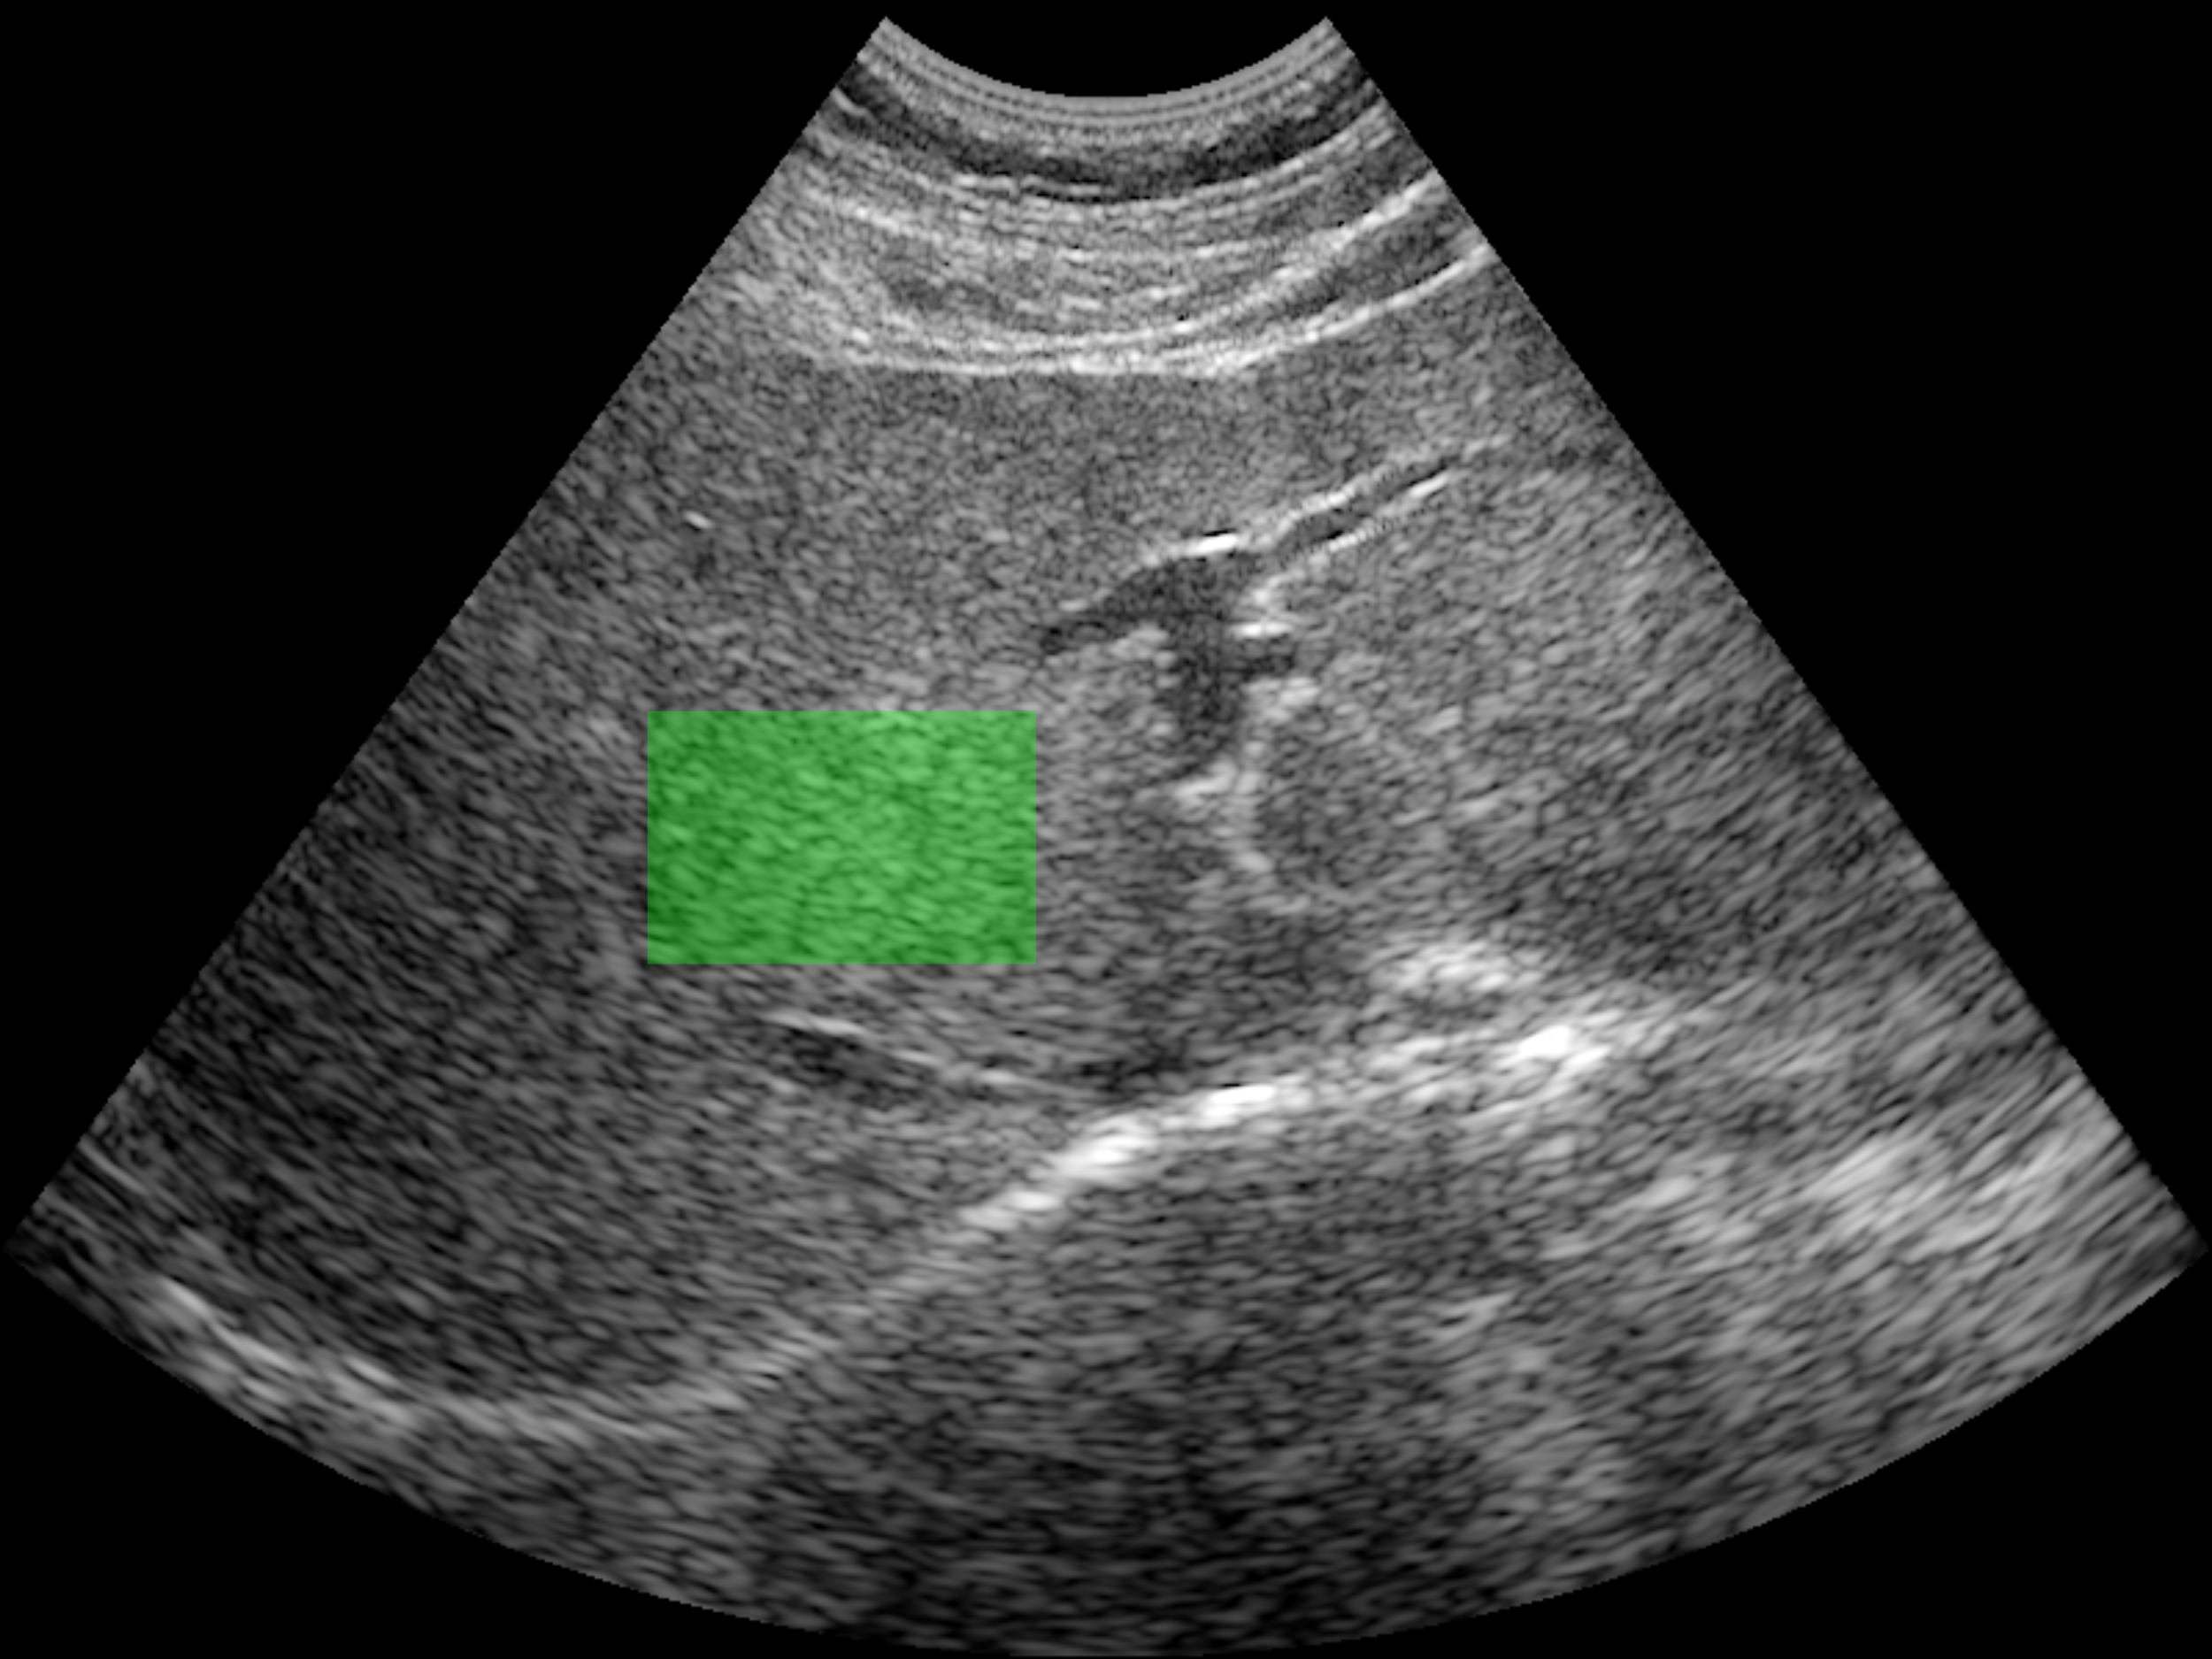
\includegraphics[height=3cm]{figures/liver_roi.png}\label{fig:liver_roi}
  }
  \subfloat[Cardiac image]{
    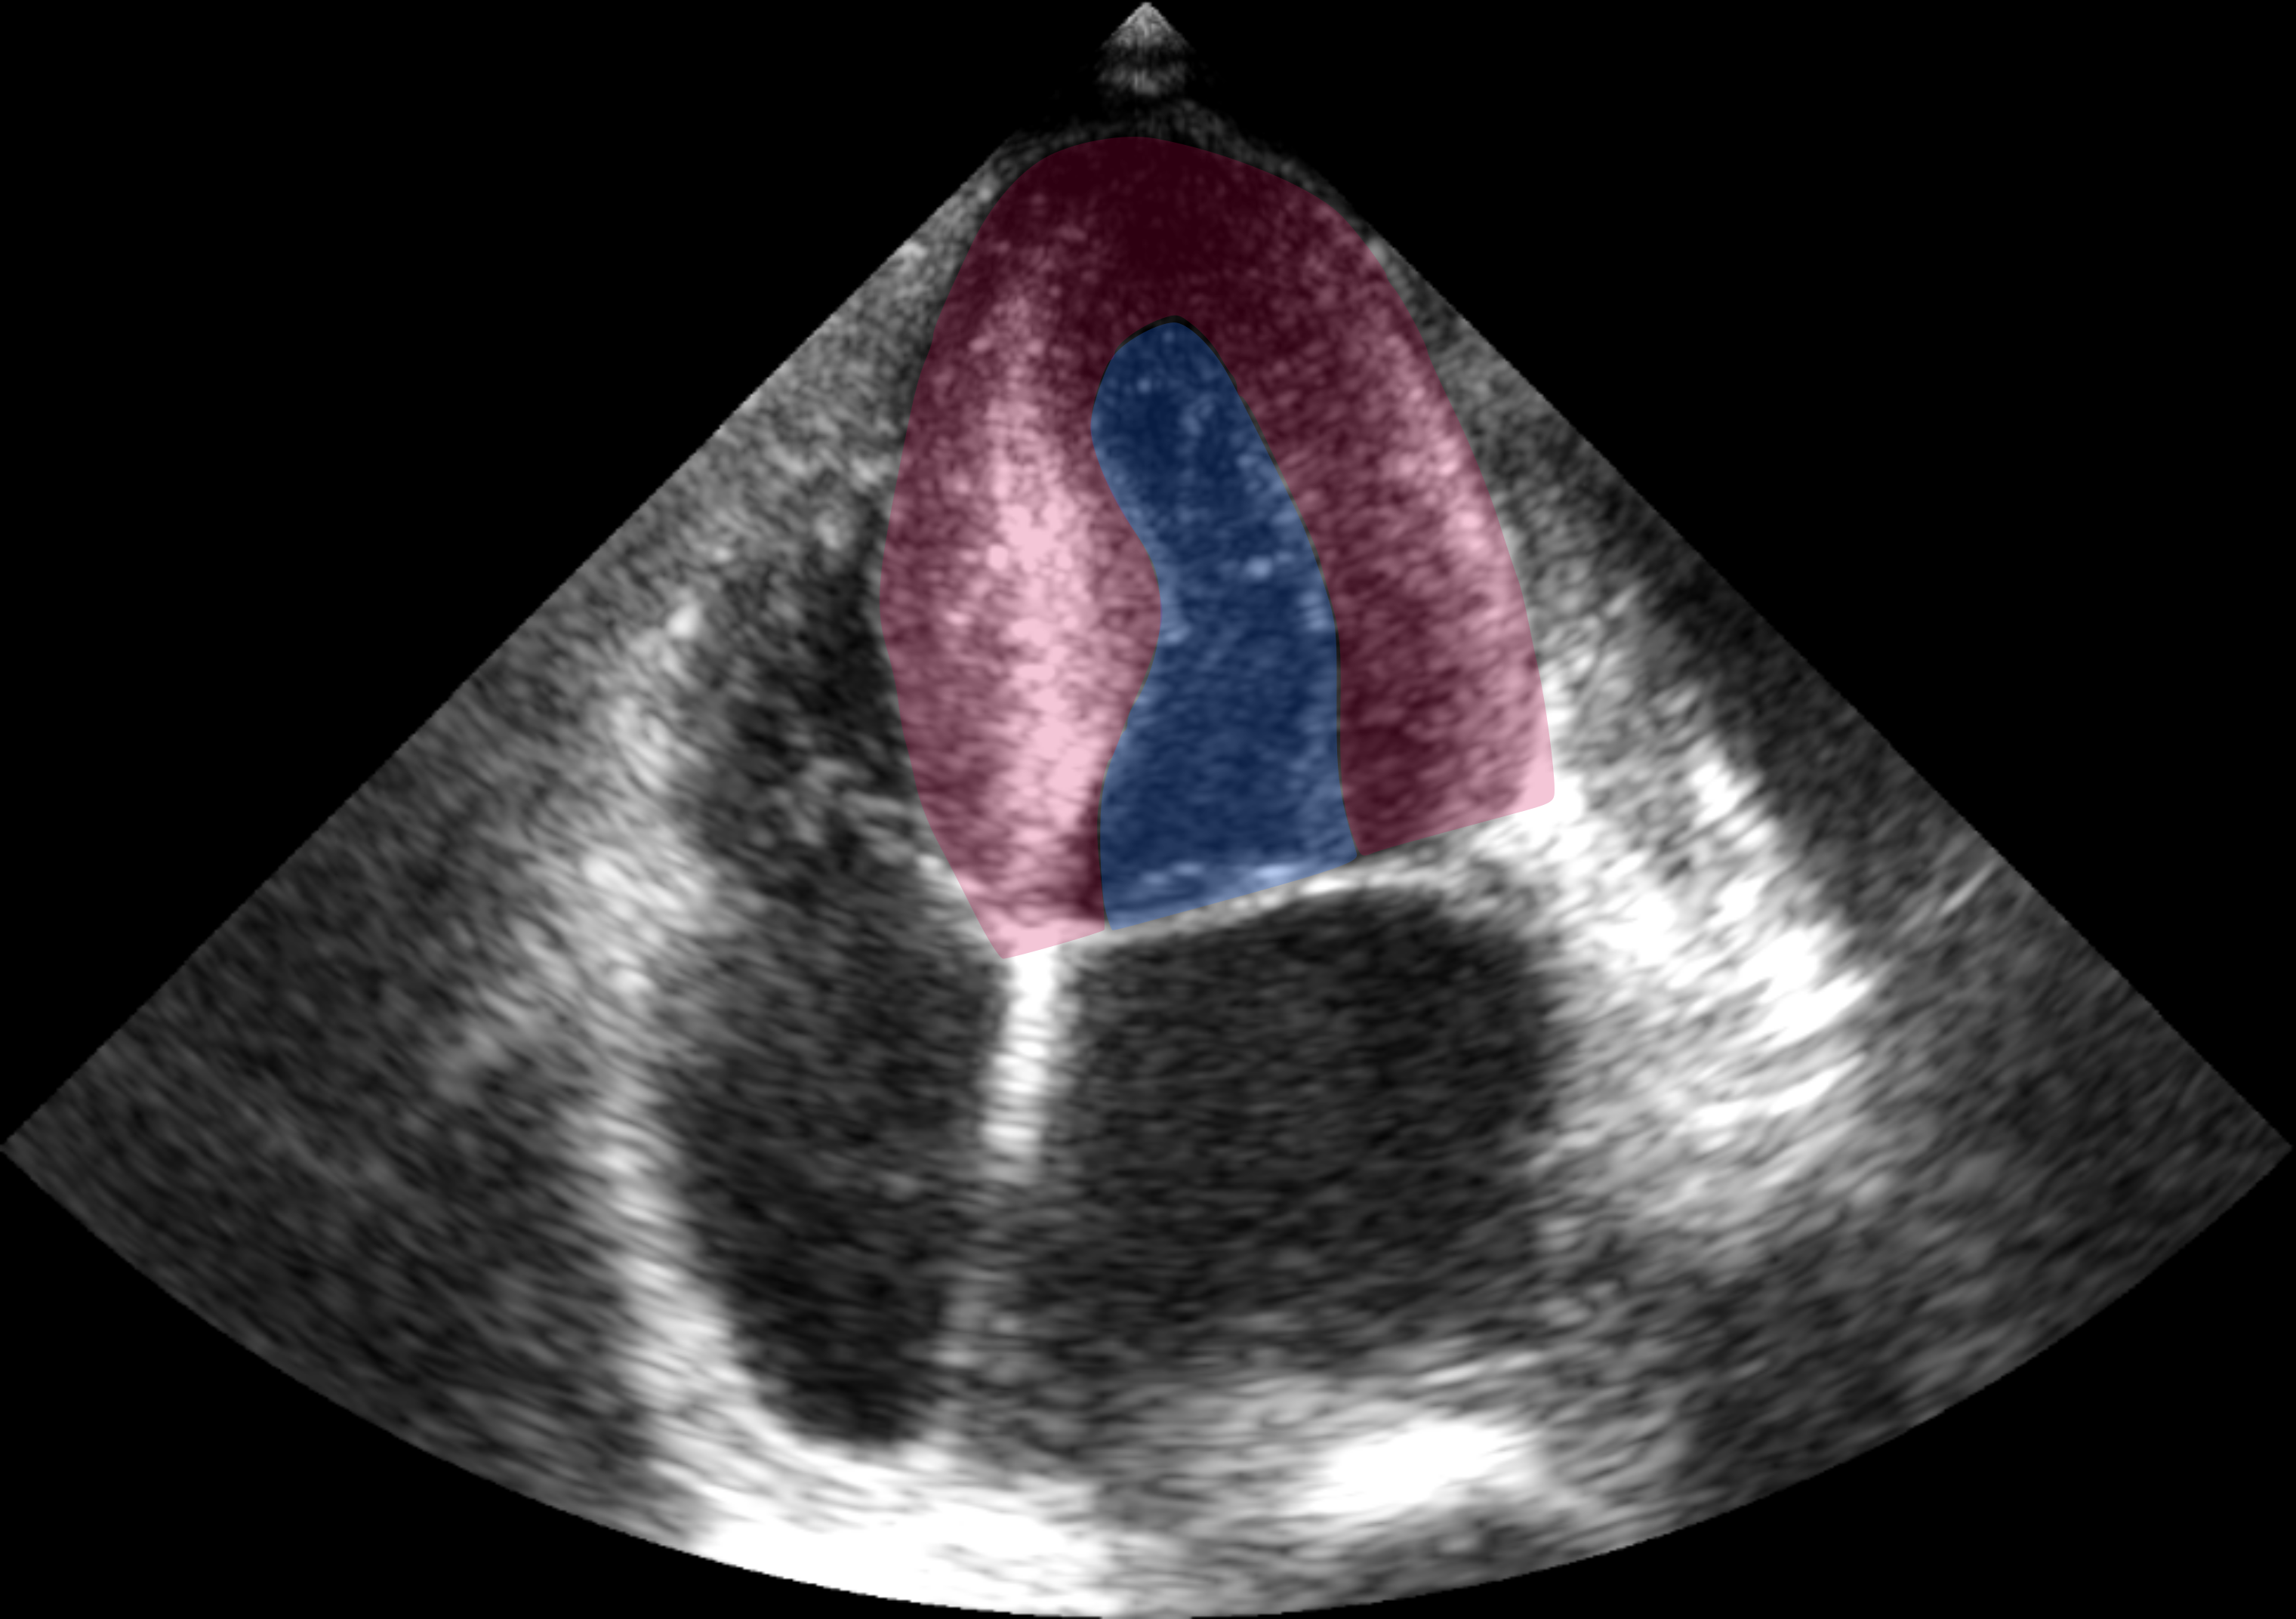
\includegraphics[height=3cm]{figures/cardiac_roi.png}\label{fig:cardiac_roi}
  }
  \caption{Regions-of-interests used for using the objective performance metrics.
    (a) The \textcolor{orange}{orange} region is used for computing the SSNR.
    (b) The \textcolor{red}{red} region (endocardium of the left ventricle) and \textcolor{blue}{blue} region (blood of the left ventricle) are used for computing the gCNR and CNR.
    The red region is also used for computing the SNR.
  }\label{fig:roi}
\end{figure}
% 
%\paragraph{Regions-of-Interests}
The regions-of-interests used for computing the performance metrics are shown in~\cref{fig:roi}.
For the liver image, we compute the metrics over multiple frames, while for the echocardiographic image, we compute the metrics only using the presented frame.


\begin{figure*}
  \centering
  \begin{subfigure}[b]{0.15\textwidth}
    \begin{tikzpicture}[
        spy using outlines={%
          rectangle,magnification=3,size=\textwidth,
          every spy on node/.append style={transparentwindow}
        }
      ]
      \node (figA) at (0.0,0.0) {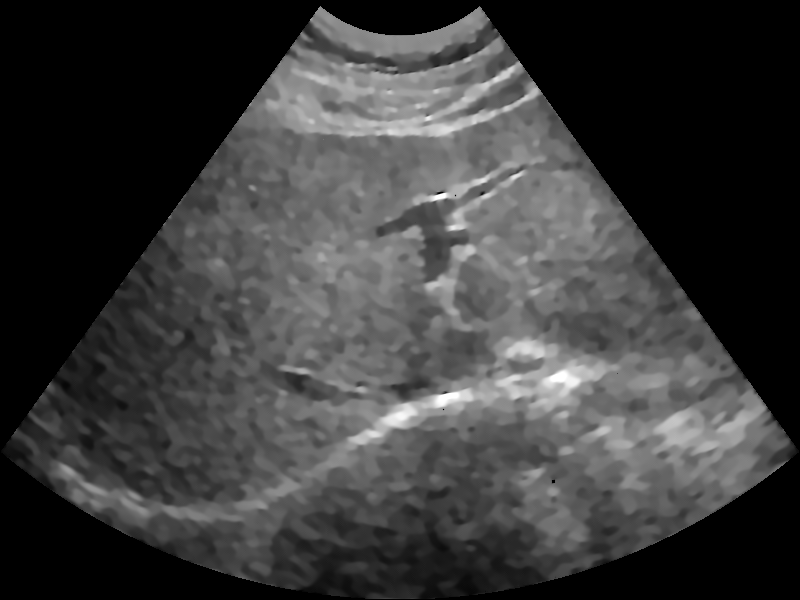
\includegraphics[width=\textwidth, trim={4cm 4cm 4cm 0cm}, clip]{figures/liver1_osrad.png}};
      \spy on (0.15, 0.0) in node [redwindow, anchor=north] at ($(figA.south)$);
    \end{tikzpicture}
    \caption{OSRAD}\label{fig:liver1_osrad}
  \end{subfigure}%
  \begin{subfigure}[b]{0.15\textwidth}
    \begin{tikzpicture}[
        spy using outlines={%
          rectangle, magnification=3,size=\textwidth,
          every spy on node/.append style={transparentwindow}
        }
      ]
      \node (figA) at (0.0,0.0) {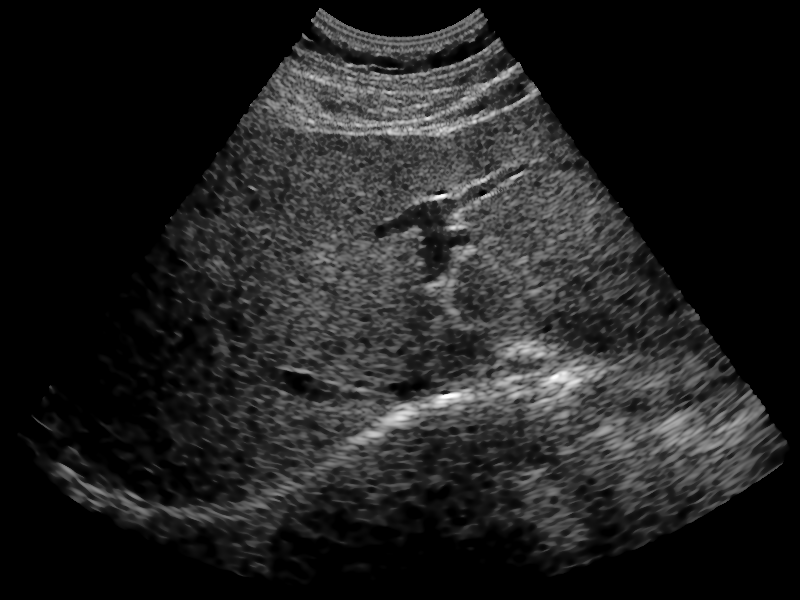
\includegraphics[width=\textwidth, trim={4cm 4cm 4cm 0cm}, clip]{figures/liver1_admss.png}};
      \spy on (0.15, 0.0) in node [redwindow, anchor=north] at ($(figA.south)$);
    \end{tikzpicture}
    \caption{ADMSS}\label{fig:liver1_admss}
  \end{subfigure}%
  \begin{subfigure}[b]{0.15\textwidth}
    \begin{tikzpicture}[
        spy using outlines={%
          rectangle, magnification=3,size=\textwidth,
          every spy on node/.append style={transparentwindow}
        }
      ]
      \node (figA) at (0.0,0.0) {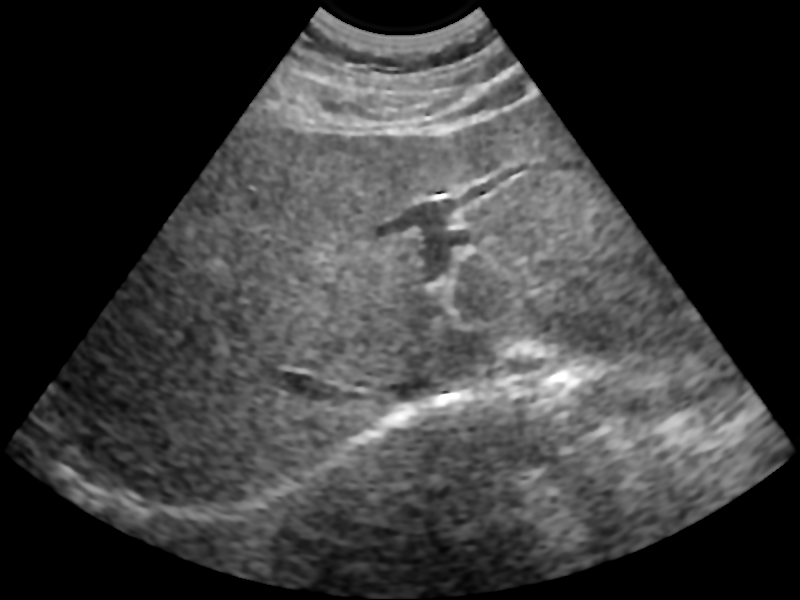
\includegraphics[width=\textwidth, trim={4cm 4cm 4cm 0cm}, clip]{figures/liver1_lpndsf.png}};
      \spy on (0.15, 0.0) in node [redwindow, anchor=north] at ($(figA.south)$);
    \end{tikzpicture}
    \caption{LPNDSF}\label{fig:liver1_lpndsf}
  \end{subfigure}%
  \begin{subfigure}[b]{0.15\textwidth}
    \begin{tikzpicture}[
        spy using outlines={%
          rectangle,magnification=3,size=\textwidth,
          every spy on node/.append style={transparentwindow}
        }
      ]
      \node (figA) at (0.0,0.0) {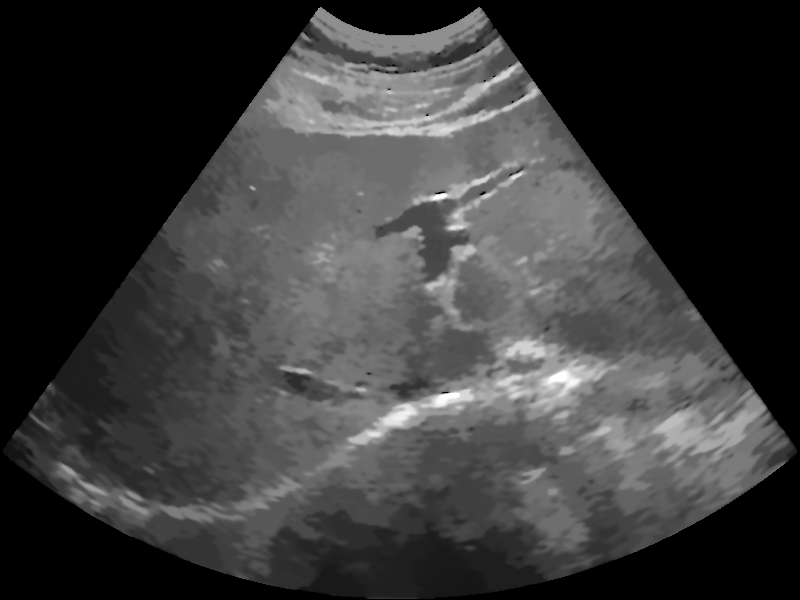
\includegraphics[width=\textwidth, trim={4cm 4cm 4cm 0cm}, clip]{figures/liver1_mnlm.png}};
      \spy on (0.15, 0.0) in node [redwindow, anchor=north] at ($(figA.south)$);
    \end{tikzpicture}
    \caption{MNLM}\label{fig:liver1_mnlm}
  \end{subfigure}%
  \begin{subfigure}[b]{0.15\textwidth}
    \begin{tikzpicture}[
        spy using outlines={%
          rectangle,magnification=3,size=\textwidth,
          every spy on node/.append style={transparentwindow}
        }
      ]
      \node (figA) at (0.0,0.0) {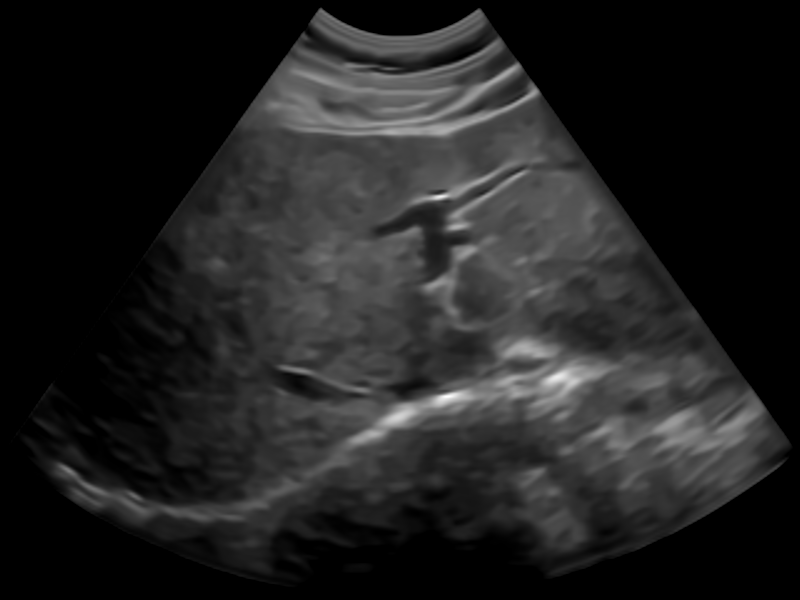
\includegraphics[width=\textwidth, trim={4cm 4cm 4cm 0cm}, clip]{figures/liver1_nllr.png}};
      \spy on (0.15, 0.0) in node [redwindow, anchor=north] at ($(figA.south)$);
    \end{tikzpicture}
    \caption{NLLR}\label{fig:liver1_nllr}
  \end{subfigure}%
  \begin{subfigure}[b]{0.15\textwidth}
    \begin{tikzpicture}[
        spy using outlines={%
          rectangle,magnification=3,size=\textwidth,
          every spy on node/.append style={transparentwindow}
        }
      ]
      \node (figA) at (0.0,0.0) {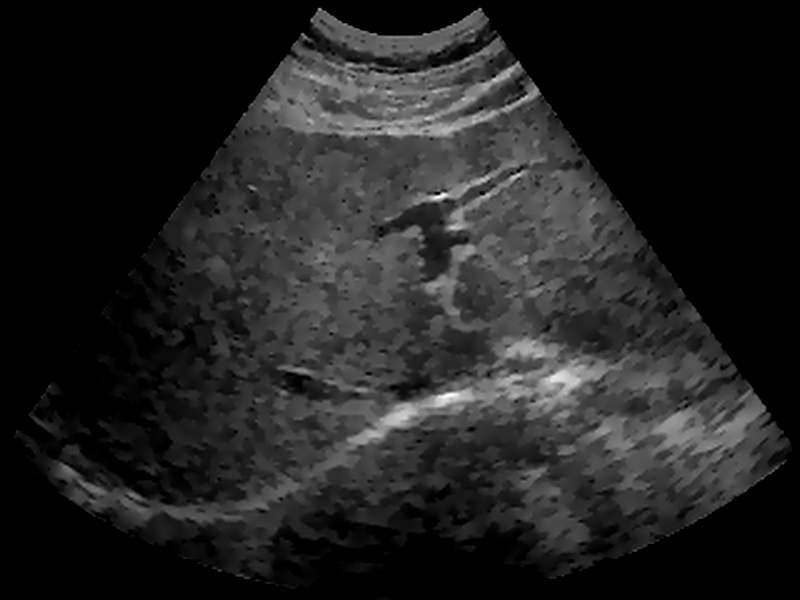
\includegraphics[width=\textwidth, trim={4cm 4cm 4cm 0cm}, clip]{figures/liver1_pfdtv.png}};
      \spy on (0.15, 0.0) in node [redwindow, anchor=north] at ($(figA.south)$);
    \end{tikzpicture}
    \caption{PFDTV}\label{fig:liver1_pfdtv}
  \end{subfigure}\\
  \begin{subfigure}[b]{0.15\textwidth}
    \begin{tikzpicture}[
        spy using outlines={%
          rectangle,magnification=3,size=\textwidth,
          every spy on node/.append style={transparentwindow}
        }
      ]
      \node (figA) at (0.0,0.0) {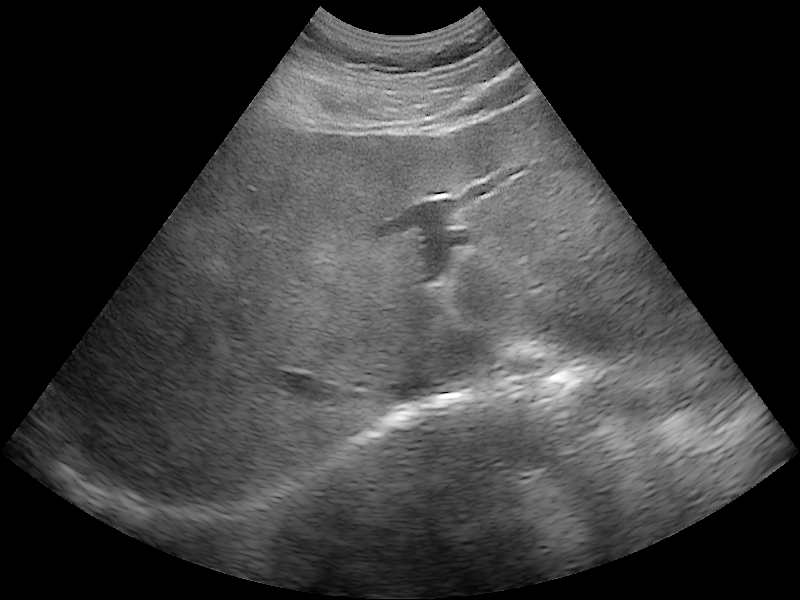
\includegraphics[width=\textwidth, trim={4cm 4cm 4cm 0cm}, clip]{figures/liver1_clpdQ.png}};
      \spy on (0.15, 0.0) in node [redwindow, anchor=north] at ($(figA.south)$);
    \end{tikzpicture}
    \caption{CLPD-SSNR}\label{fig:liver1_clpdssnr}
  \end{subfigure}%
  \begin{subfigure}[b]{0.15\textwidth}
    \begin{tikzpicture}[
        spy using outlines={%
          rectangle,magnification=3,size=\textwidth,
          every spy on node/.append style={transparentwindow}
        }
      ]
      \node (figA) at (0.0,0.0) {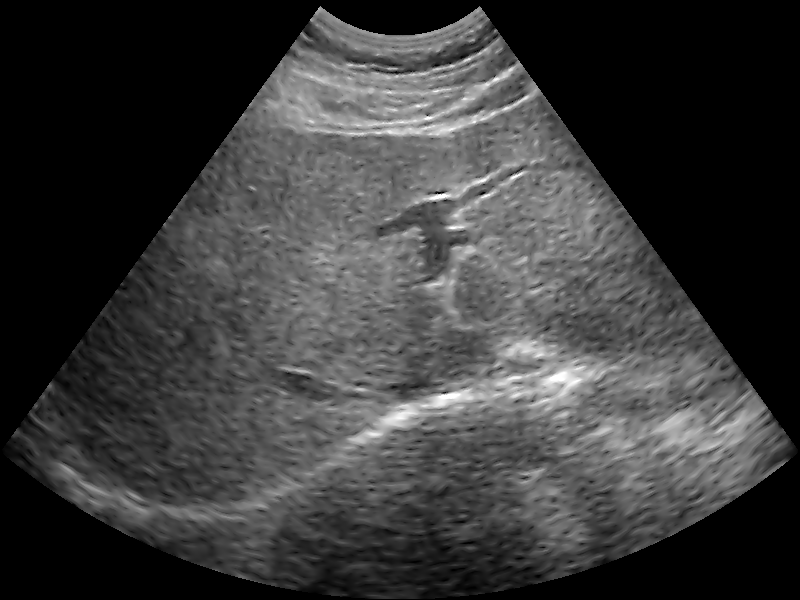
\includegraphics[width=\textwidth, trim={4cm 4cm 4cm 0cm}, clip]{figures/liver1_clpda.png}};
      \spy on (0.15, 0.0) in node [redwindow, anchor=north] at ($(figA.south)$);
    \end{tikzpicture}
    \caption{CLPD-A}\label{fig:liver1_clpda}
  \end{subfigure}%
  \begin{subfigure}[b]{0.15\textwidth}
    \begin{tikzpicture}[
        spy using outlines={%
          rectangle,magnification=3,size=\textwidth,
          every spy on node/.append style={transparentwindow}
        }
      ]
      \node (figA) at (0.0,0.0) {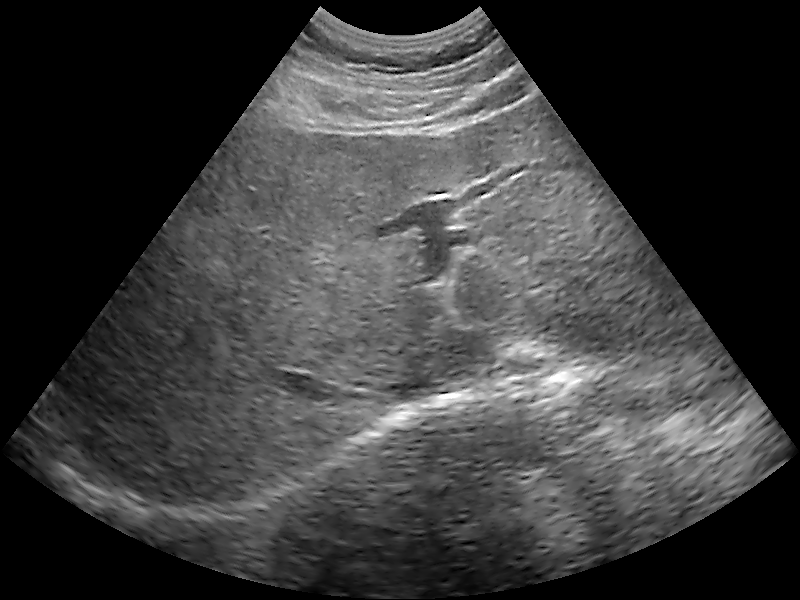
\includegraphics[width=\textwidth, trim={4cm 4cm 4cm 0cm}, clip]{figures/liver1_clpdb.png}};
      \spy on (0.15, 0.0) in node [redwindow, anchor=north] at ($(figA.south)$);
    \end{tikzpicture}
    \caption{CLPD-B}\label{fig:liver1_clpdb}
  \end{subfigure}%
  \begin{subfigure}[b]{0.15\textwidth}
    \begin{tikzpicture}[
        spy using outlines={%
          rectangle,magnification=3,size=\textwidth,
          every spy on node/.append style={transparentwindow}
        }
      ]
      \node (figA) at (0.0,0.0) {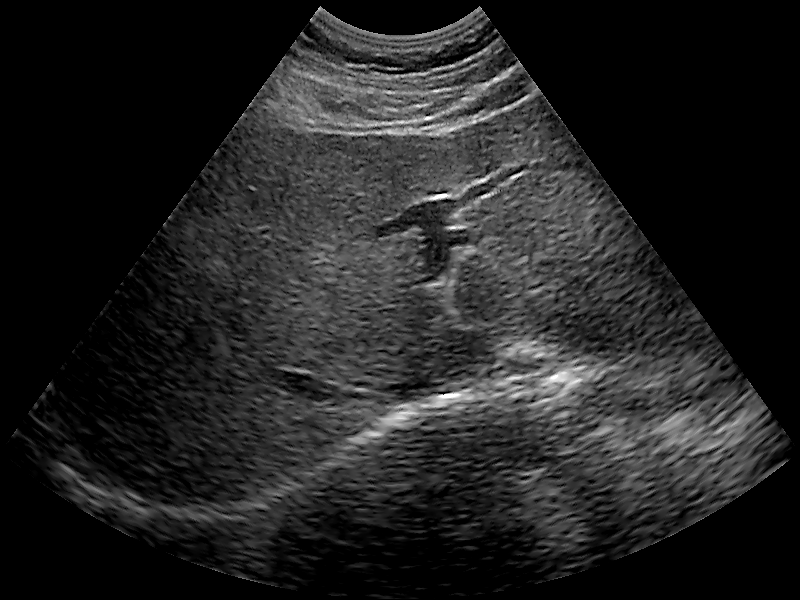
\includegraphics[width=\textwidth, trim={4cm 4cm 4cm 0cm}, clip]{figures/liver1_clpdc.png}};
      \spy on (0.15, 0.0) in node [redwindow, anchor=north] at ($(figA.south)$);
    \end{tikzpicture}
    \caption{CLPD-C}\label{fig:liver1_clpdc}
  \end{subfigure}%
  \begin{subfigure}[b]{0.15\textwidth}
    \begin{tikzpicture}[
        spy using outlines={%
          rectangle,magnification=3,size=\textwidth,
          every spy on node/.append style={transparentwindow}
        }
      ]
      \node (figA) at (0.0,0.0) {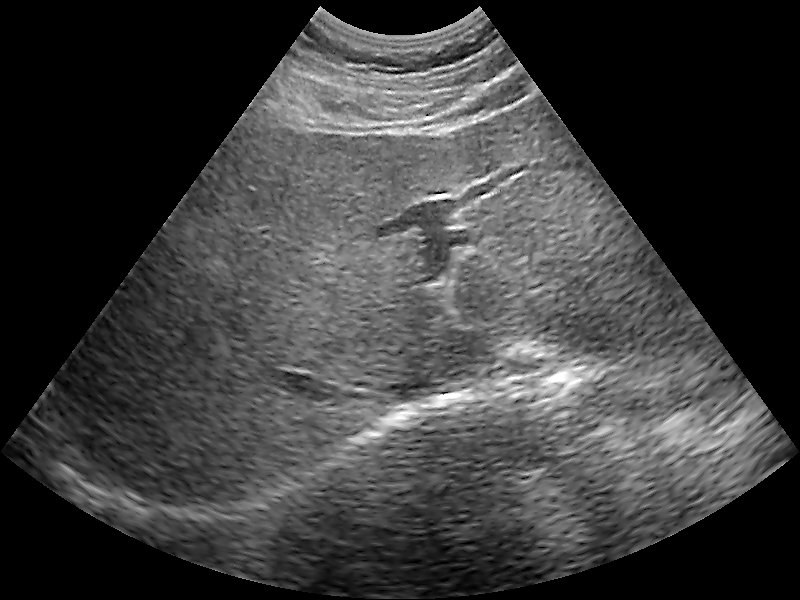
\includegraphics[width=\textwidth, trim={4cm 4cm 4cm 0cm}, clip]{figures/liver1_clpdd.png}};
      \spy on (0.15, 0.0) in node [redwindow, anchor=north] at ($(figA.south)$);
    \end{tikzpicture}
    \caption{CLPD-D}\label{fig:liver1_clpdd}
  \end{subfigure}%
  \begin{subfigure}[b]{0.15\textwidth}
    \begin{tikzpicture}[
        spy using outlines={%
          rectangle,magnification=3,size=\textwidth,
          every spy on node/.append style={redwindow}
        }
      ]
      \node (figA) at (0.0,0.0) {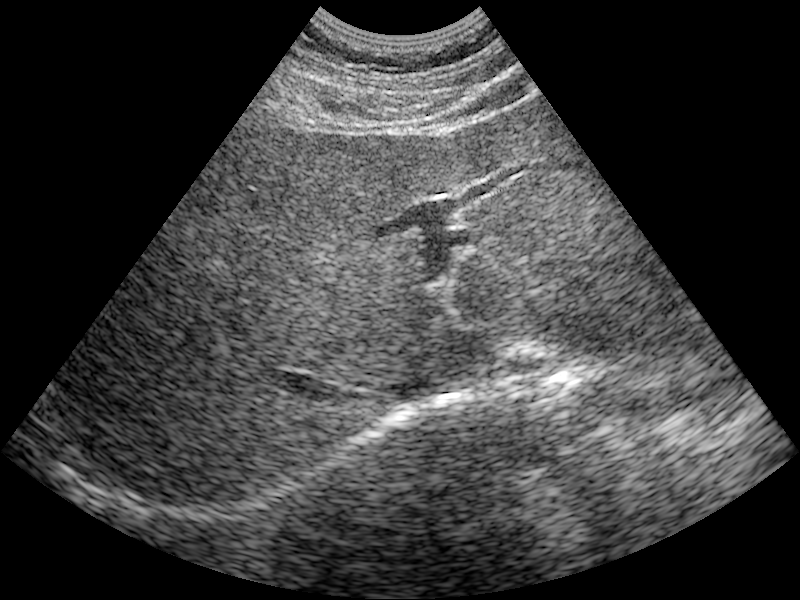
\includegraphics[width=\textwidth, trim={4cm 4cm 4cm 0cm}, clip]{figures/liver1.png}};
      \spy on (0.15, 0.0) in node [redwindow, anchor=north] at ($(figA.south)$);
    \end{tikzpicture}
    \caption{Original}\label{fig:liver_original}
  \end{subfigure}
  \caption{Results on a liver subcostal-view image.}\label{fig:liver1}
\end{figure*}

%%% Local Variables:
%%% TeX-master: "master"
%%% End:

%
\begin{table}
  \centering
  \caption{Quantatitive Results on a Liver Subcostal View}\label{table:liver1}
  \begin{threeparttable}
  \setlength{\tabcolsep}{3.5pt}
  \begin{tabular}{llrrr}
    \toprule
    & \multicolumn{1}{c}{\textbf{Algorithm}}
    & \multicolumn{1}{c}{\textbf{SSNR} \texttt{[dB]}}
    & \multicolumn{1}{c}{\textbf{SSIM}}
    & \multicolumn{1}{c}{\(\mathbf{S_{3}}\)} \\\midrule
    \multirow{6}{*}{\footnotesize{Baselines}} & OSRAD & \textbf{20.8 {\tiny(20.3, 21.2)}} & 0.792 {\tiny(0.791, 0.794)} & 0.476 {\tiny(0.473, 0.481)}\\
    & ADMSS & 16.9 {\tiny(16.5, 17.4)} & \textbf{0.927 {\tiny(0.893, 0.963)}} & 0.350 {\tiny(0.347, 0.353)} \\
    & LPNDSF & 19.7 {\tiny(19.4, 20.0)} & 0.763 {\tiny(0.762, 0.764)}         & 0.343 {\tiny(0.340, 0.346)} \\
    & MNLM & \textbf{22.1 {\tiny(21.6, 22.7)}} & 0.811 {\tiny(0.809, 0.812)}  & 0.033 {\tiny(0.329, 0.342)} \\
    & NLLR & \textbf{22.0 {\tiny(21.6, 22.5)}} & 0.764 {\tiny(0.762, 0.765)}  & 0.141 {\tiny(0.140, 0.142)} \\
    & PFDTV & \textbf{20.0 {\tiny(19.6, 20.4)}} & 0.822 {\tiny(0.820, 0.823)} & 0.461 {\tiny(0.456, 0.465)} \\
    \midrule
    \multirow{5}{*}{\footnotesize{This work}} & CLPD-{\scriptsize{SSNR}}  & \textbf{21.0 {\tiny(20.7, 21.4)}} & \textbf{0.914 {\tiny(0.913, 0.914)}} & \textbf{0.509 {\tiny(0.507, 0.511)}} \\
    & CLPD-A  & 19.9 {\tiny(19.6, 20.2)} & 0.883 {\tiny(0.882, 0.884)} & \textbf{0.490 {\tiny(0.486, 0.494)}} \\
    & CLPD-B  & 19.8 {\tiny(19.6, 20.2)} & \textbf{0.913 {\tiny(0.913, 0.914)}} & \textbf{0.507 {\tiny(0.503, 0.511)}} \\
    & CLPD-C  & 18.2 {\tiny(18.0, 18.5)} & \textbf{0.954 {\tiny(0.953, 0.954)}} & \textbf{0.587 {\tiny(0.581, 0.592)}} \\
    & CLPD-D & 19.0 {\tiny(18.7, 19.3)} & \textbf{0.933 {\tiny(0.932, 0.933)}} &  \textbf{0.565 {\tiny(0.562, 0.569)}} \\\bottomrule
  \end{tabular}
  \begin{tablenotes}
    \item[*] We report the average, 10\%, and \%90 percentiles of the metrics taken over 16 frames.
    \item[*] The performance of the top 5 algorithms for each metric are shown in bold face.
  \end{tablenotes}
  \end{threeparttable}
\end{table}
%
\subsection{Results on Liver Subcostal View}
We first present experimental results with a liver subcostal view image sequence.
For this experiment, we also include a CLPD setting tuned to maximize both the SSNR and SSIM metric using vanilla BO, denoted as CLPD-SSNR.

\subsubsection{Qualitative Results}
A single frame processed by each method is shown in~\cref{fig:liver1}.

%\paragraph{Speckle reduction}
The CLPDs tuned by sonographers (CLPD-A to CLPD-D) did not show significant speckle reduction.
Notice the contrast with CLPD-SSNR, which has been tuned to obtain the least speckle.
This shows that, for sonographers, speckle reduction is less relevant to the clinical quality of liver images.
Among the CLDPs tuned by sonographers, CLPD-B shows the least speckle, reflecting the preferential difference among sonographers.
On the other hand, MNLM, NLLR showed the least speckle, but NLLR results in very blurry images.

When focusing on blurriness and clarity, the expert tuned CLPDs showed the best results.
The edges of the left portal vein are noticibly sharper on CLPD-C and CLPD-D.
In contrast, most of the considered baselines except for ADMSS and MNLM are notibly blurry.
Meanwhile, OSRAD, LPNDSF, and PFDTV resulted in ``blocky'' patterns, possibly because of the strong presence of pepper noise. 
Especially, ADMSS showed \textit{increased} speckle due to peppers.
The probabilstic model of ADMSS missspecified peppers as background, resulting in their enlargation.


\begin{figure*}
  \vspace{-0.2in}
  \centering
  \begin{subfigure}[b]{0.15\textwidth}
    \begin{tikzpicture}[
        spy using outlines={%
          rectangle,magnification=3,size=\textwidth,
          every spy on node/.append style={transparentwindow}
        }
      ]
      \node (figA) at (0.0,0.0) {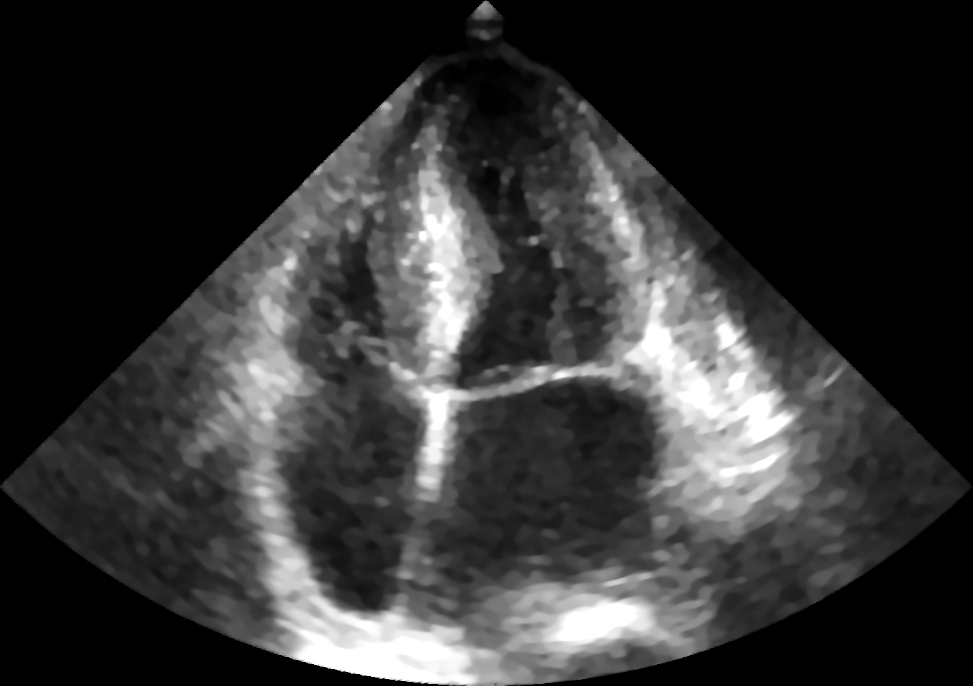
\includegraphics[width=\textwidth]{figures/cardiac3_osrad.png}};
      \spy on (0.1, 0.2) in node [redwindow, anchor=north] at ($(figA.south)$);
    \end{tikzpicture}
    \caption{OSRAD}
  \end{subfigure}%
  \begin{subfigure}[b]{0.15\textwidth}
    \begin{tikzpicture}[
        spy using outlines={%
          rectangle, magnification=3,size=\textwidth,
          every spy on node/.append style={transparentwindow}
        }
      ]
      \node (figA) at (0.0,0.0) {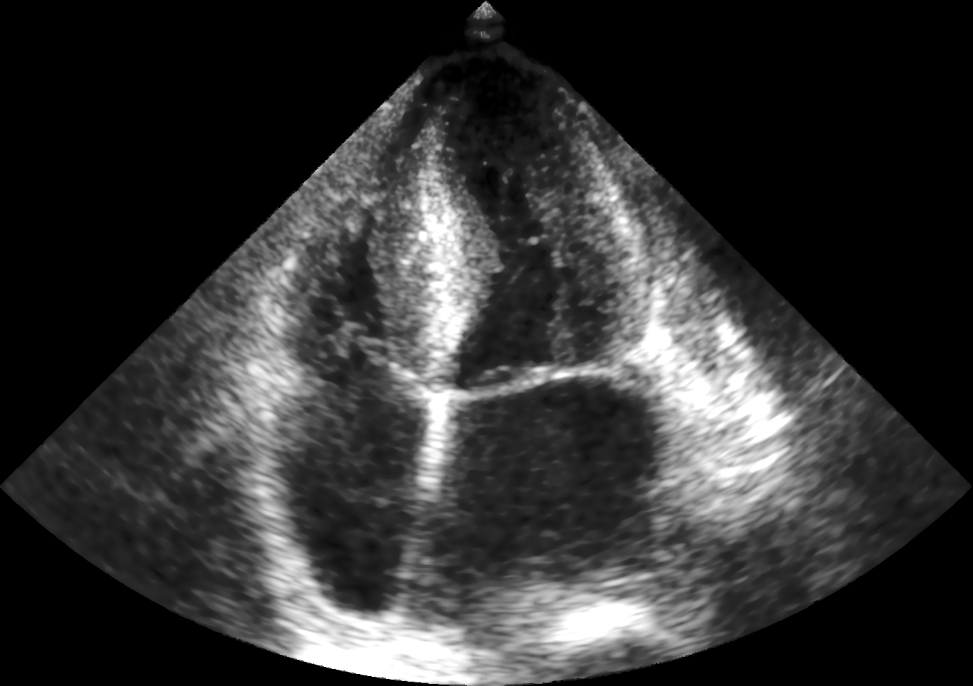
\includegraphics[width=\textwidth]{figures/cardiac3_admss.png}};
      \spy on (0.1, 0.2) in node [redwindow, anchor=north] at ($(figA.south)$);
    \end{tikzpicture}
    \caption{ADMSS}
  \end{subfigure}%
  \begin{subfigure}[b]{0.15\textwidth}
    \begin{tikzpicture}[
        spy using outlines={%
          rectangle, magnification=3,size=\textwidth,
          every spy on node/.append style={transparentwindow}
        }
      ]
      \node (figA) at (0.0,0.0) {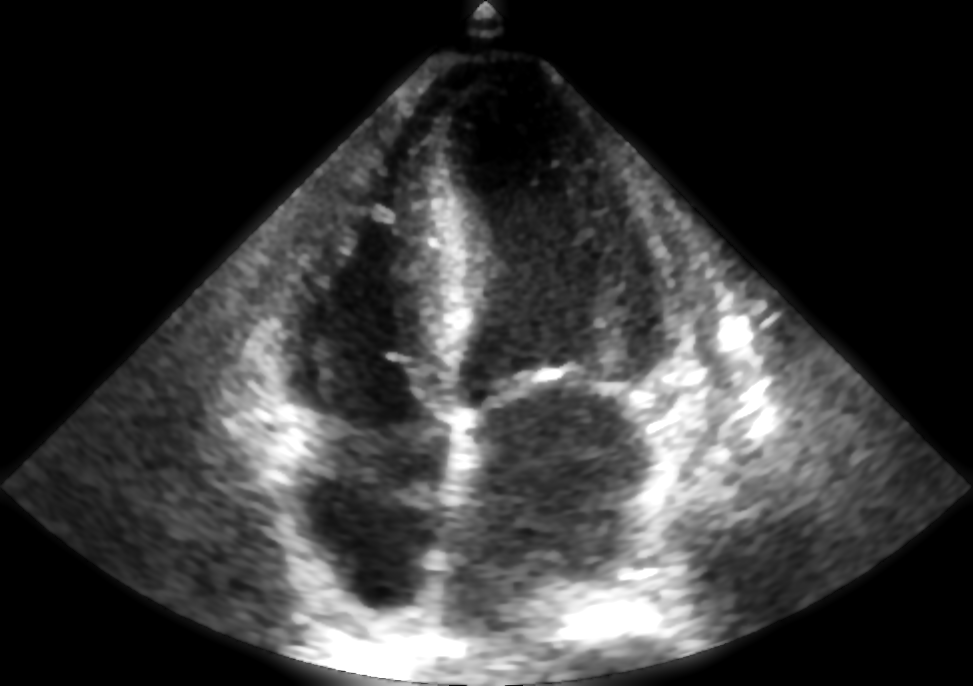
\includegraphics[width=\textwidth]{figures/cardiac3_lpndsf.png}};
      \spy on (0.1, 0.2) in node [redwindow, anchor=north] at ($(figA.south)$);
    \end{tikzpicture}
    \caption{LPNDSF}
  \end{subfigure}%
  \begin{subfigure}[b]{0.15\textwidth}
    \begin{tikzpicture}[
        spy using outlines={%
          rectangle,magnification=3,size=\textwidth,
          every spy on node/.append style={transparentwindow}
        }
      ]
      \node (figA) at (0.0,0.0) {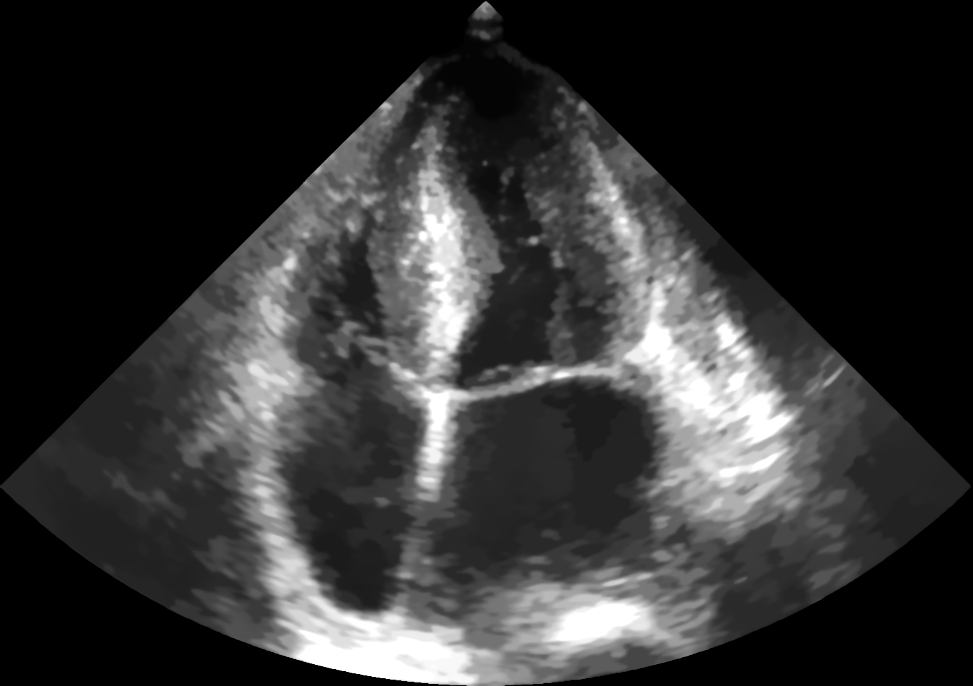
\includegraphics[width=\textwidth]{figures/cardiac3_mnlm.png}};
      \spy on (0.1, 0.2) in node [redwindow, anchor=north] at ($(figA.south)$);
    \end{tikzpicture}
    \caption{MNLM}
  \end{subfigure}%
  \begin{subfigure}[b]{0.15\textwidth}
    \begin{tikzpicture}[
        spy using outlines={%
          rectangle,magnification=3,size=\textwidth,
          every spy on node/.append style={transparentwindow}
        }
      ]
      \node (figA) at (0.0,0.0) {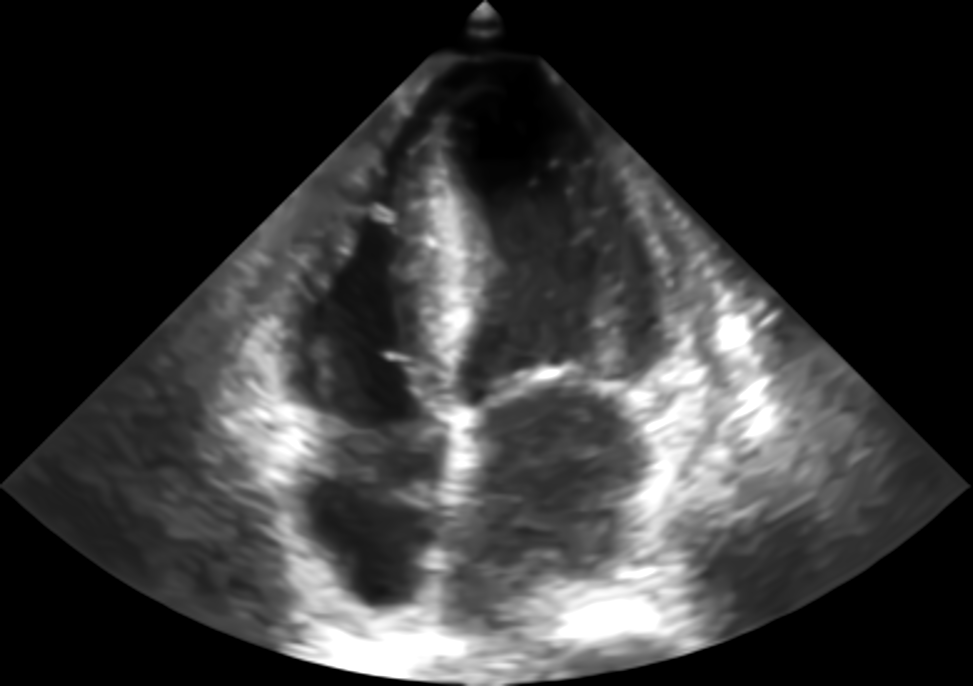
\includegraphics[width=\textwidth]{figures/cardiac3_nllr.png}};
      \spy on (0.1, 0.2) in node [redwindow, anchor=north] at ($(figA.south)$);
    \end{tikzpicture}
    \caption{NLLR}
  \end{subfigure}%
  \begin{subfigure}[b]{0.15\textwidth}
    \begin{tikzpicture}[
        spy using outlines={%
          rectangle,magnification=3,size=\textwidth,
          every spy on node/.append style={transparentwindow}
        }
      ]
      \node (figA) at (0.0,0.0) {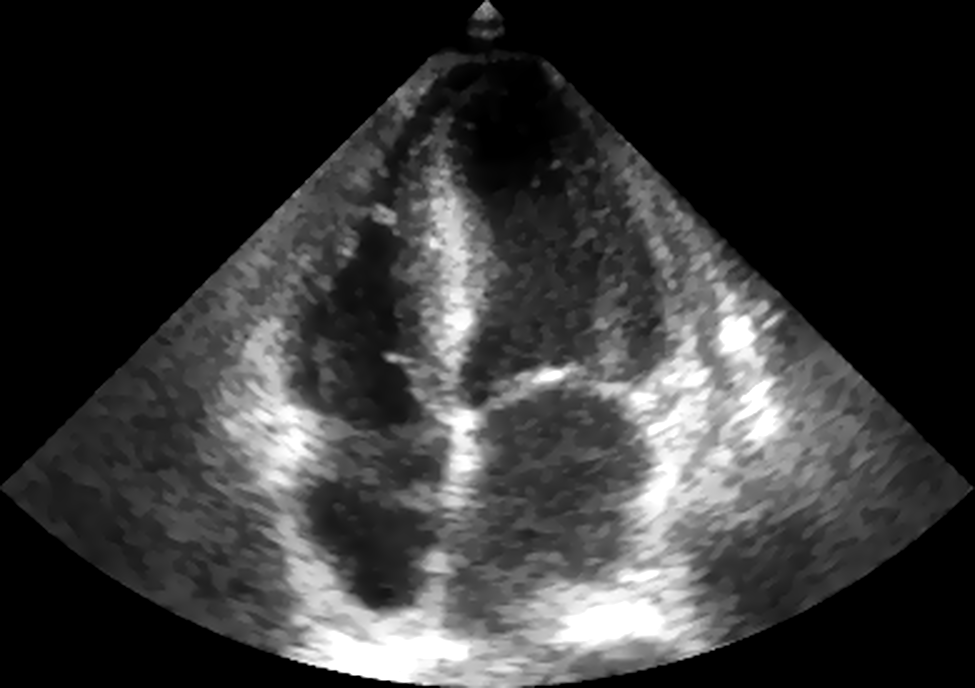
\includegraphics[width=\textwidth]{figures/cardiac3_pfdtv.png}};
      \spy on (0.1, 0.2) in node [redwindow, anchor=north] at ($(figA.south)$);
    \end{tikzpicture}
    \caption{PFDTV}
  \end{subfigure}\\
  %% \begin{subfigure}[b]{0.15\textwidth}
  %%   \begin{tikzpicture}[
  %%       spy using outlines={%
  %%         rectangle,magnification=3,size=\textwidth,
  %%         every spy on node/.append style={transparentwindow}
  %%       }
  %%     ]
  %%     \node (figA) at (0.0,0.0) {\includegraphics[width=\textwidth, trim={4cm 4cm 4cm 0cm}, clip]{figures/cardiac3_clpdQ.png}};
  %%     \spy on (0.1, 0.2) in node [redwindow, anchor=north] at ($(figA.south)$);
  %%   \end{tikzpicture}
  %%   \caption{CLPD-SSNR}
  %% \end{subfigure}%
  \begin{subfigure}[b]{0.15\textwidth}
    \begin{tikzpicture}[
        spy using outlines={%
          rectangle,magnification=3,size=\textwidth,
          every spy on node/.append style={transparentwindow}
        }
      ]
      \node (figA) at (0.0,0.0) {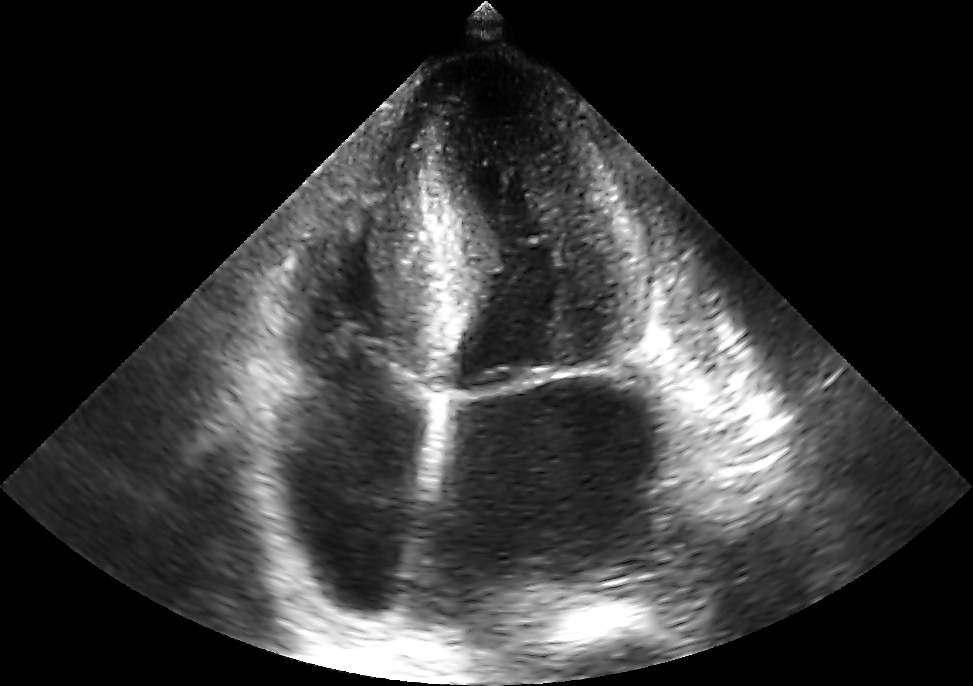
\includegraphics[width=\textwidth]{figures/cardiac3_clpda.png}};
      \spy on (0.1, 0.2) in node [redwindow, anchor=north] at ($(figA.south)$);
    \end{tikzpicture}
    \caption{CLPD-A}
  \end{subfigure}%
  \begin{subfigure}[b]{0.15\textwidth}
    \begin{tikzpicture}[
        spy using outlines={%
          rectangle,magnification=3,size=\textwidth,
          every spy on node/.append style={transparentwindow}
        }
      ]
      \node (figA) at (0.0,0.0) {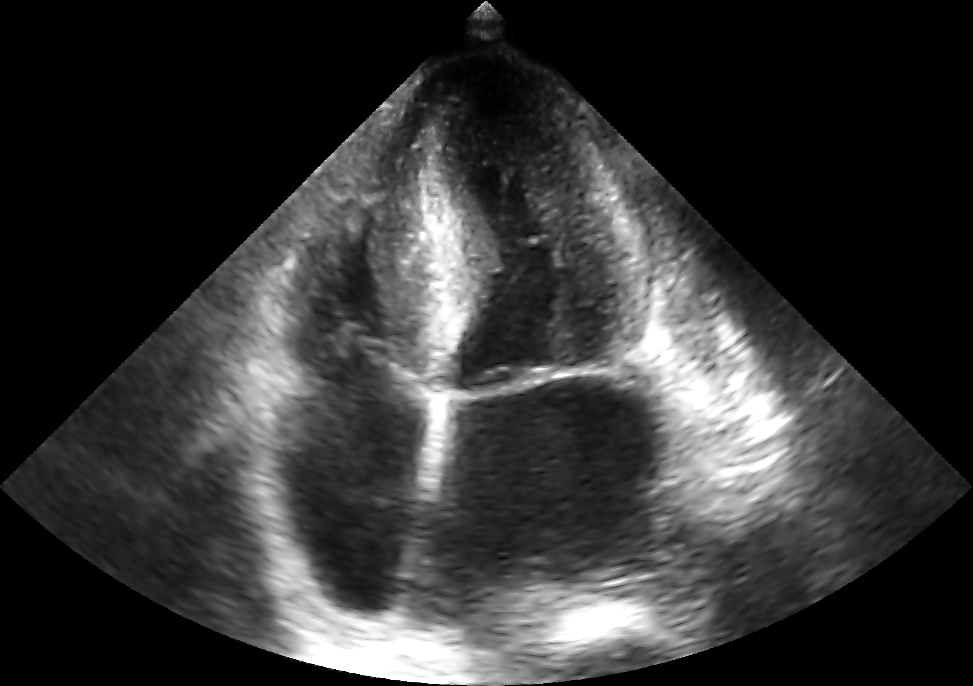
\includegraphics[width=\textwidth]{figures/cardiac3_clpdb.png}};
      \spy on (0.1, 0.2) in node [redwindow, anchor=north] at ($(figA.south)$);
    \end{tikzpicture}
    \caption{CLPD-B}
  \end{subfigure}%
  \begin{subfigure}[b]{0.15\textwidth}
    \begin{tikzpicture}[
        spy using outlines={%
          rectangle,magnification=3,size=\textwidth,
          every spy on node/.append style={transparentwindow}
        }
      ]
      \node (figA) at (0.0,0.0) {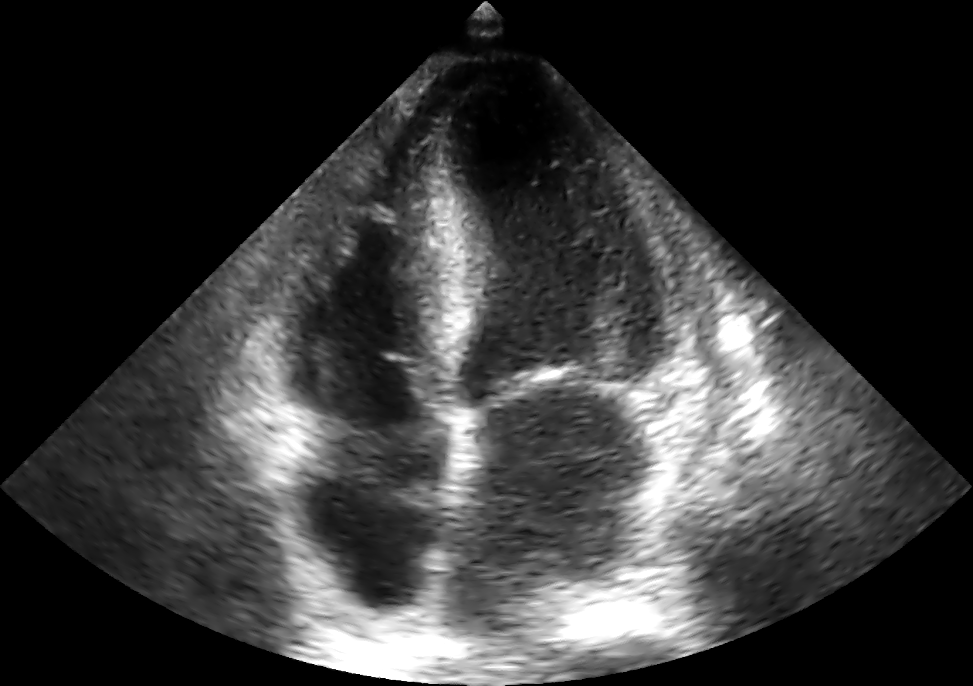
\includegraphics[width=\textwidth]{figures/cardiac3_clpde.png}};
      \spy on (0.1, 0.2) in node [redwindow, anchor=north] at ($(figA.south)$);
    \end{tikzpicture}
    \caption{CLPD-E}
  \end{subfigure}%
  \begin{subfigure}[b]{0.15\textwidth}
    \begin{tikzpicture}[
        spy using outlines={%
          rectangle,magnification=3,size=\textwidth,
          every spy on node/.append style={transparentwindow}
        }
      ]
      \node (figA) at (0.0,0.0) {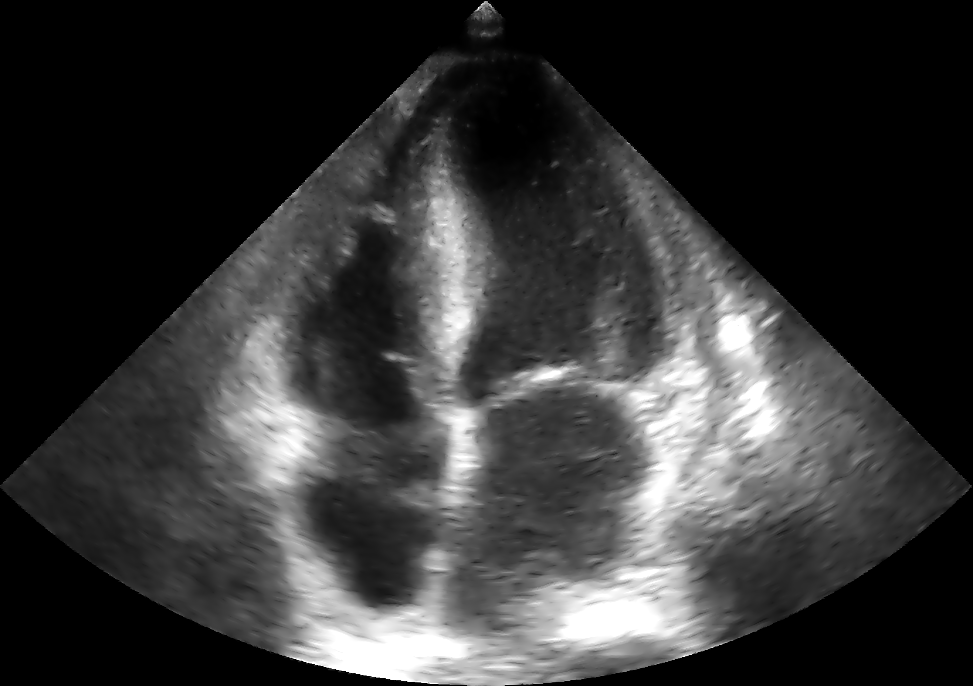
\includegraphics[width=\textwidth]{figures/cardiac3_clpdf.png}};
      \spy on (0.1, 0.2) in node [redwindow, anchor=north] at ($(figA.south)$);
    \end{tikzpicture}
    \caption{CLPD-F}
  \end{subfigure}%
  \begin{subfigure}[b]{0.15\textwidth}
    \begin{tikzpicture}[
        spy using outlines={%
          rectangle,magnification=3,size=\textwidth,
          every spy on node/.append style={redwindow}
        }
      ]
      \node (figA) at (0.0,0.0) {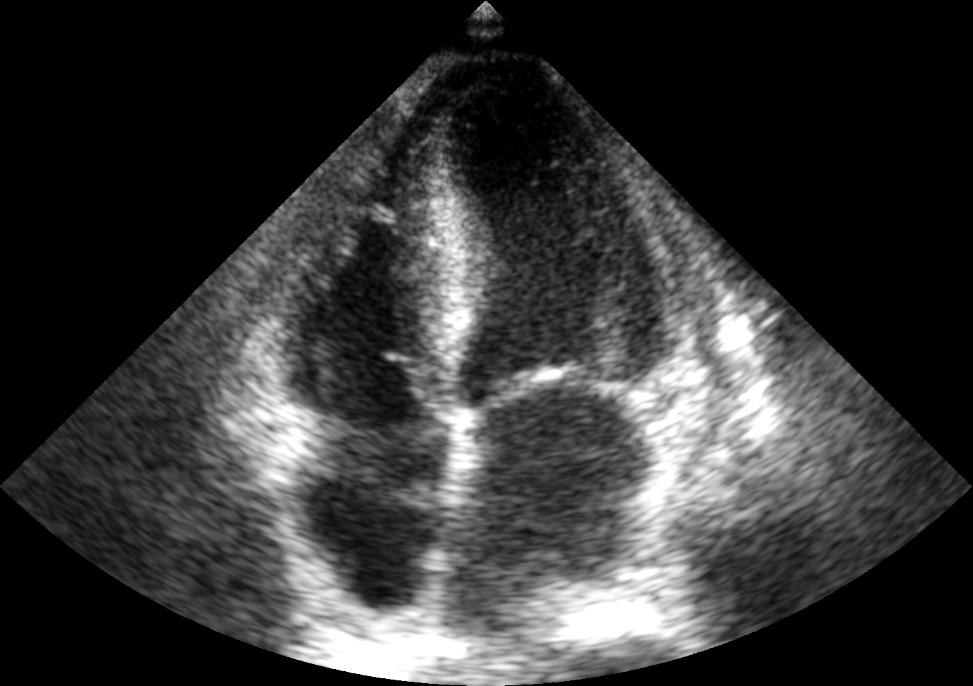
\includegraphics[width=\textwidth]{figures/cardiac3.png}};
      \spy on (0.1, 0.2) in node [redwindow, anchor=north] at ($(figA.south)$);
    \end{tikzpicture}
    \caption{Original}\label{fig:cardiac3_original}
  \end{subfigure}
  \caption{
    Results on echocardiographic 4-chamber view.
    The red squares are zooming on the left-ventricle.
  }\label{fig:cardiac3}
  \vspace{-0.15in}
\end{figure*}

%
\subsubsection{Quantitative Results}
The quantatitive results using objective performance metrics are shown in~\cref{table:liver1}.
First, we can see that the SSNR values obtained using the CLPDs are worse compared to the baselines except for CLPD-obj., which is natural since it was explicitly tuned to obtain a high SSNR.
This shows that, while it is definitely possible to obtain a high SSNR with the CLPD, none of the sonographers preferred a high SSNR.
Instead, they preferred to preserve some level of speckle noise.
In contrast, all of the baselines except for ADMSS obtained higher SSNR.
In particular, the MNLM obtains the highest leverl of SSNR, which supports the statement that non-local means methods are excellent at removing speckle (which is unfortunately, not desirable).

Meanwhile, when looking at other metrics than the SSNR, the results look quite different.
The CLPDs obtained both high SSIM and high \(S_3\) overall.
Only ADMSS obtained a high SSIM, which is natural since it refrains diffusing tissues.
CLPDs on the other hand all resulted in high levels of SSIMs, which shows that sonographers strongly prefer images that do not look different from the original image.

Lastly, when looking at the \(S_3\) metric, we can see that all CLPDs obtained much higher values.
This shows that the CLPD is capable of conserving sharpness, and that sonographers strongly prefer sharp-looking images.
In fact, many of the participating sonographers explicitly stated that they ``do not want to trade sharpness for less speckle''.
Our results clearly reflect this sentiment.
For this reason, while the NLLR is very good at reinforcing strucutres and reducing speckle, it results in images that are significantly blurry both qualititatively and quantitatively (according to \(S_3\)), which limits its clinical value.

\begin{table}
  \centering
  \caption{Quantatitive Results on Echocardiographic 4-Chamber View}\label{table:cardiac3}
  \setlength{\tabcolsep}{3pt}
  \begin{threeparttable}
  \begin{tabular}{llrrrrr}
    \toprule
    & \multicolumn{1}{c}{\textbf{Algorithm}}
    & \multicolumn{1}{c}{\textbf{gCNR}}
    & \multicolumn{1}{c}{\textbf{CNR}}
    & \multicolumn{1}{c}{\textbf{SNR}}
    & \multicolumn{1}{c}{\textbf{SSIM}}
    & \multicolumn{1}{c}{\(\mathbf{S_{3}}\)}\\
    & \multicolumn{1}{c}{}
    & \multicolumn{1}{c}{}
    & \texttt{[dB]}
    & \texttt{[dB]}
    & \multicolumn{1}{c}{}
    & \multicolumn{1}{c}{} \\\midrule
    \multirow{6}{*}{Baselines}
    & OSRAD  & 0.490          & -1.62          & 4.51          & 0.891          & 0.500 \\
    & ADMSS  & 0.467          & -1.67          & 4.33          & \textbf{0.967} & 0.204 \\
    & LPNDSF & 0.473          & -1.67          & 4.39          & 0.868          & 0.458 \\
    & MNLM   & \textbf{0.534} & \textbf{-1.61} & 4.42          & 0.918          & 0.414 \\
    & NLLR   & \textbf{0.501} & \textbf{-1.60} & 4.61          & 0.857          & 0.042\\
    & PFDTV  & 0.480          & -1.65          & 4.49          & 0.865          & 0.155 \\\midrule
    \multirow{4}{*}{This work}
    & CLPD-A & 0.484          & -1.64          & \textbf{4.64} & \textbf{0.957} & \textbf{0.858} \\
    & CLPD-B & \textbf{0.496} & \textbf{-1.55} & \textbf{4.69} & \textbf{0.949} & \textbf{0.685} \\
    & CLPD-E & 0.476          & -1.63          & \textbf{4.61} & \textbf{0.961} & \textbf{0.507} \\
    & CLPD-F & \textbf{0.507} & \textbf{-1.50} & \textbf{4.79} & 0.920          & \textbf{0.705} \\\bottomrule
  \end{tabular}
  \begin{tablenotes}
    \item[*] The performance of the top 4 algorithms for each metric are shown in bold face.
  \end{tablenotes}
  \end{threeparttable}
\end{table}
%

\begin{figure*}
  \vspace{-0.1in}
  \centering
  \begin{subfigure}[b]{0.15\textwidth}
    \begin{tikzpicture}[
        spy using outlines={%
          rectangle,magnification=3,size=\textwidth,
          every spy on node/.append style={transparentwindow}
        }
      ]
      \node (figA) at (0.0,0.0) {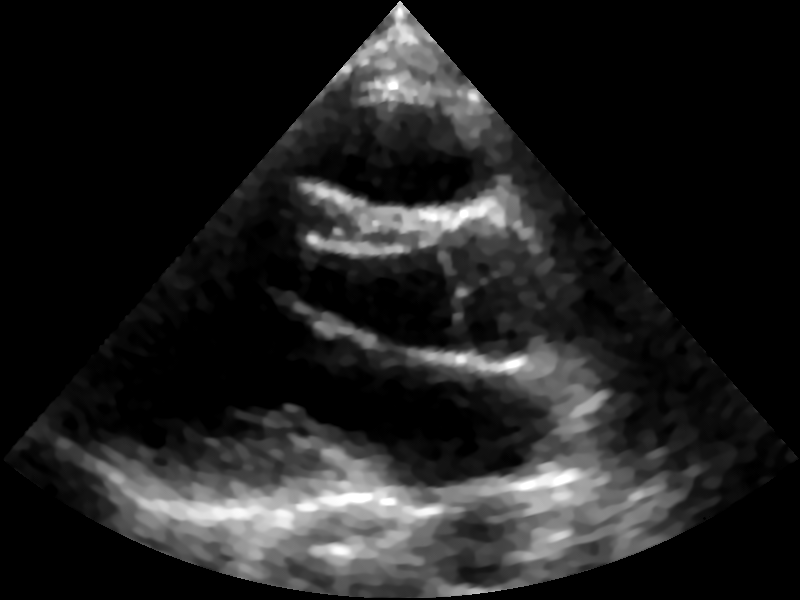
\includegraphics[width=\textwidth]{figures/cardiac1_osrad.png}};
      \spy on (0.05, 0.05) in node [redwindow, anchor=north] at ($(figA.south)$);
    \end{tikzpicture}
    \caption{OSRAD}
  \end{subfigure}%
  \begin{subfigure}[b]{0.15\textwidth}
    \begin{tikzpicture}[
        spy using outlines={%
          rectangle, magnification=3,size=\textwidth,
          every spy on node/.append style={transparentwindow}
        }
      ]
      \node (figA) at (0.0,0.0) {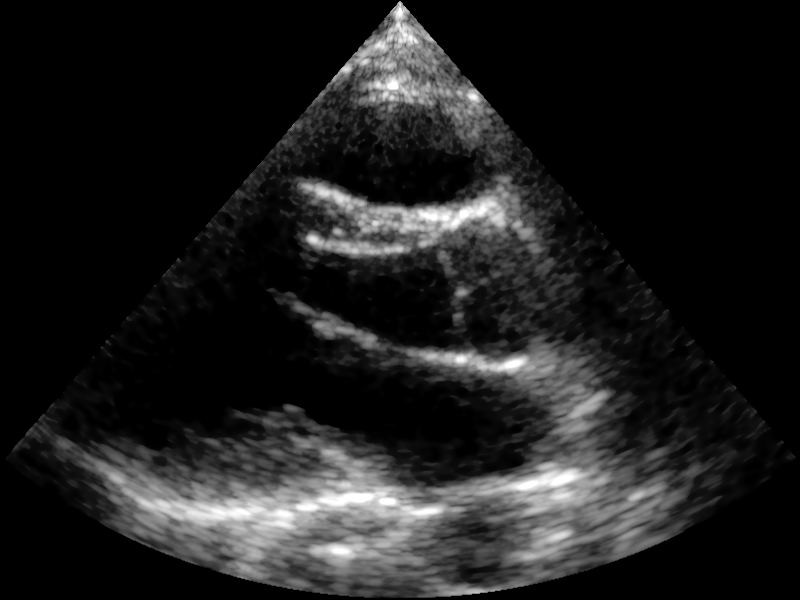
\includegraphics[width=\textwidth]{figures/cardiac1_admss.png}};
      \spy on (0.05, 0.05) in node [redwindow, anchor=north] at ($(figA.south)$);
    \end{tikzpicture}
    \caption{ADMSS}
  \end{subfigure}%
  \begin{subfigure}[b]{0.15\textwidth}
    \begin{tikzpicture}[
        spy using outlines={%
          rectangle, magnification=3,size=\textwidth,
          every spy on node/.append style={transparentwindow}
        }
      ]
      \node (figA) at (0.0,0.0) {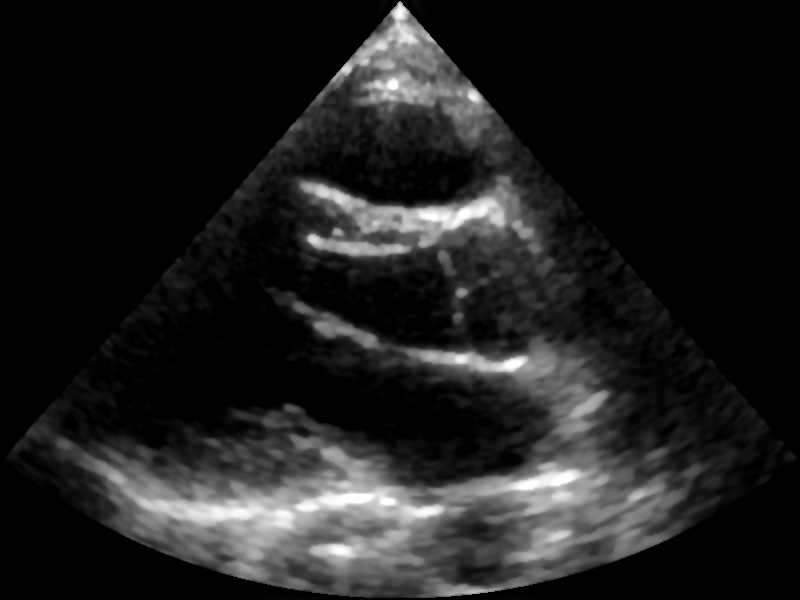
\includegraphics[width=\textwidth]{figures/cardiac1_lpndsf.png}};
      \spy on (0.05, 0.05) in node [redwindow, anchor=north] at ($(figA.south)$);
    \end{tikzpicture}
    \caption{LPNDSF}
  \end{subfigure}%
  \begin{subfigure}[b]{0.15\textwidth}
    \begin{tikzpicture}[
        spy using outlines={%
          rectangle,magnification=3,size=\textwidth,
          every spy on node/.append style={transparentwindow}
        }
      ]
      \node (figA) at (0.0,0.0) {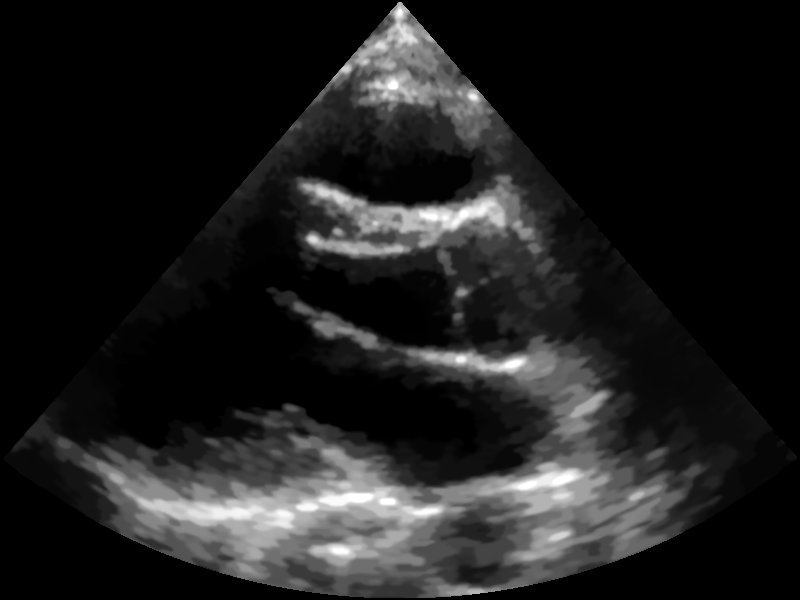
\includegraphics[width=\textwidth]{figures/cardiac1_mnlm.png}};
      \spy on (0.05, 0.05) in node [redwindow, anchor=north] at ($(figA.south)$);
    \end{tikzpicture}
    \caption{MNLM}
  \end{subfigure}%
  \begin{subfigure}[b]{0.15\textwidth}
    \begin{tikzpicture}[
        spy using outlines={%
          rectangle,magnification=3,size=\textwidth,
          every spy on node/.append style={transparentwindow}
        }
      ]
      \node (figA) at (0.0,0.0) {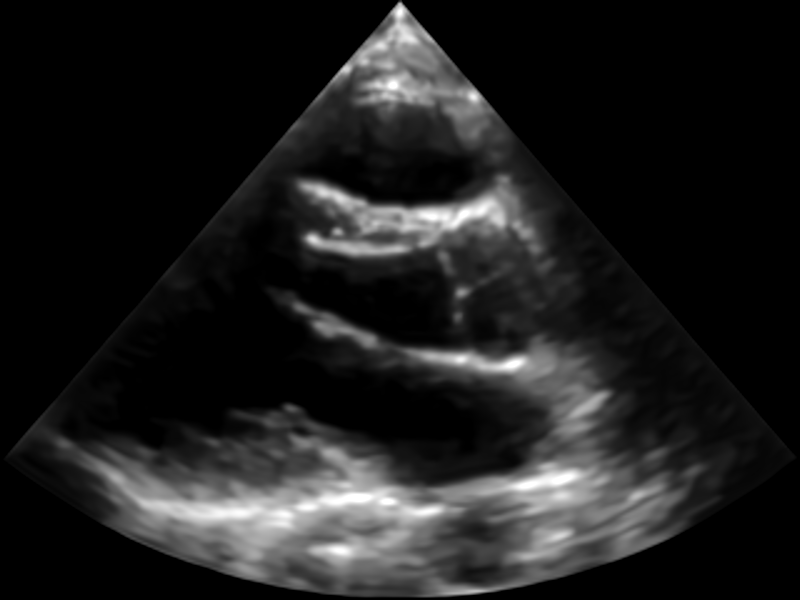
\includegraphics[width=\textwidth]{figures/cardiac1_nllr.png}};
      \spy on (0.05, 0.05) in node [redwindow, anchor=north] at ($(figA.south)$);
    \end{tikzpicture}
    \caption{NLLR}
  \end{subfigure}%
  \begin{subfigure}[b]{0.15\textwidth}
    \begin{tikzpicture}[
        spy using outlines={%
          rectangle,magnification=3,size=\textwidth,
          every spy on node/.append style={transparentwindow}
        }
      ]
      \node (figA) at (0.0,0.0) {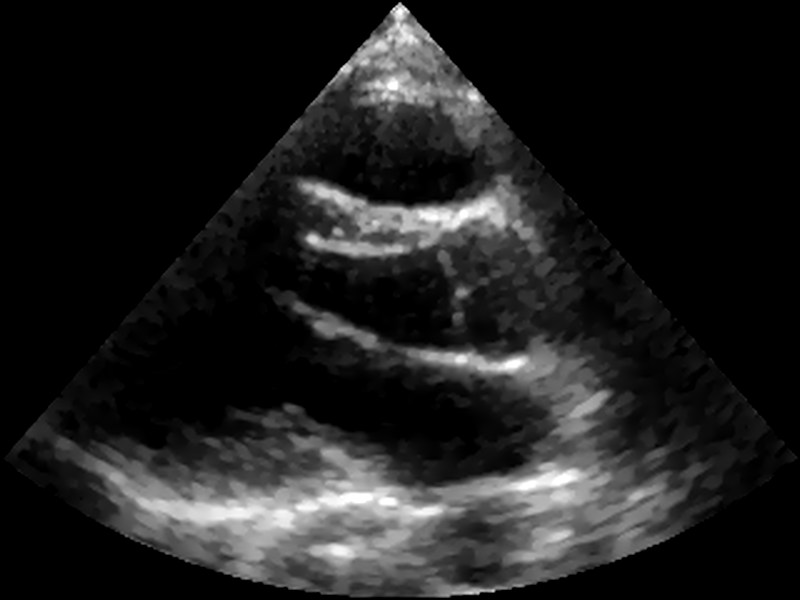
\includegraphics[width=\textwidth]{figures/cardiac1_pfdtv.png}};
      \spy on (0.05, 0.05) in node [redwindow, anchor=north] at ($(figA.south)$);
    \end{tikzpicture}
    \caption{PFDTV}
  \end{subfigure}\\
  %% \begin{subfigure}[b]{0.15\textwidth}
  %%   \begin{tikzpicture}[
  %%       spy using outlines={%
  %%         rectangle,magnification=3,size=\textwidth,
  %%         every spy on node/.append style={transparentwindow}
  %%       }
  %%     ]
  %%     \node (figA) at (0.0,0.0) {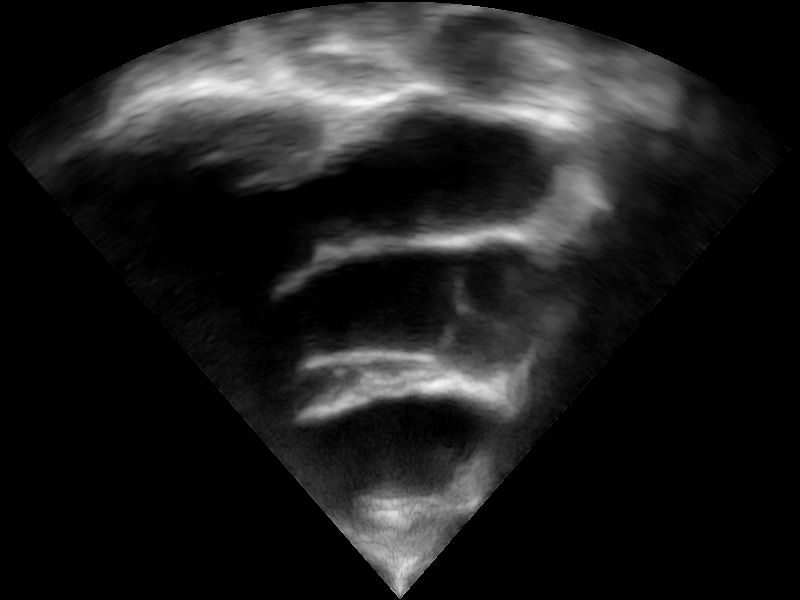
\includegraphics[width=\textwidth, trim={4cm 4cm 4cm 0cm}, clip]{figures/cardiac1_clpdQ.png}};
  %%     \spy on (0.05, 0.05) in node [redwindow, anchor=north] at ($(figA.south)$);
  %%   \end{tikzpicture}
  %%   \caption{CLPD-SSNR}
  %% \end{subfigure}%
  \begin{subfigure}[b]{0.15\textwidth}
    \begin{tikzpicture}[
        spy using outlines={%
          rectangle,magnification=3,size=\textwidth,
          every spy on node/.append style={transparentwindow}
        }
      ]
      \node (figA) at (0.0,0.0) {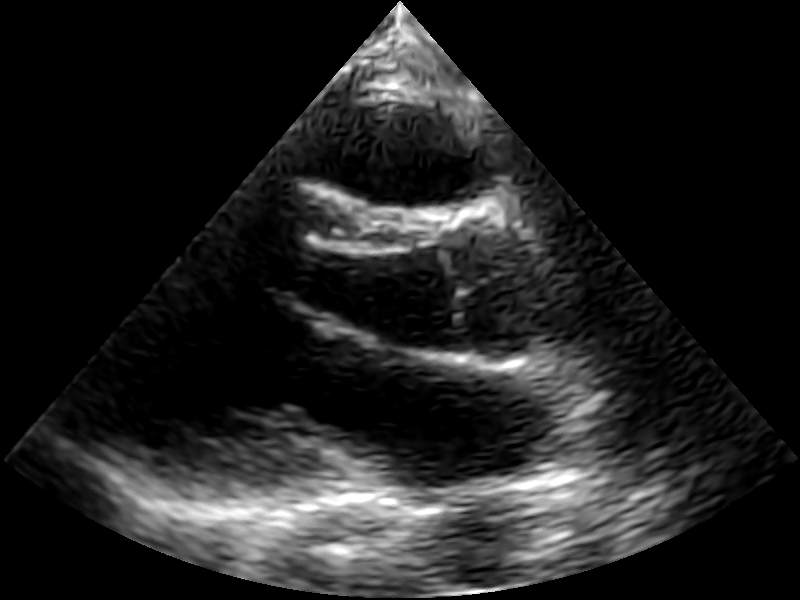
\includegraphics[width=\textwidth]{figures/cardiac1_clpda.png}};
      \spy on (0.05, 0.05) in node [redwindow, anchor=north] at ($(figA.south)$);
    \end{tikzpicture}
    \caption{CLPD-A}
  \end{subfigure}%
  \begin{subfigure}[b]{0.15\textwidth}
    \begin{tikzpicture}[
        spy using outlines={%
          rectangle,magnification=3,size=\textwidth,
          every spy on node/.append style={transparentwindow}
        }
      ]
      \node (figA) at (0.0,0.0) {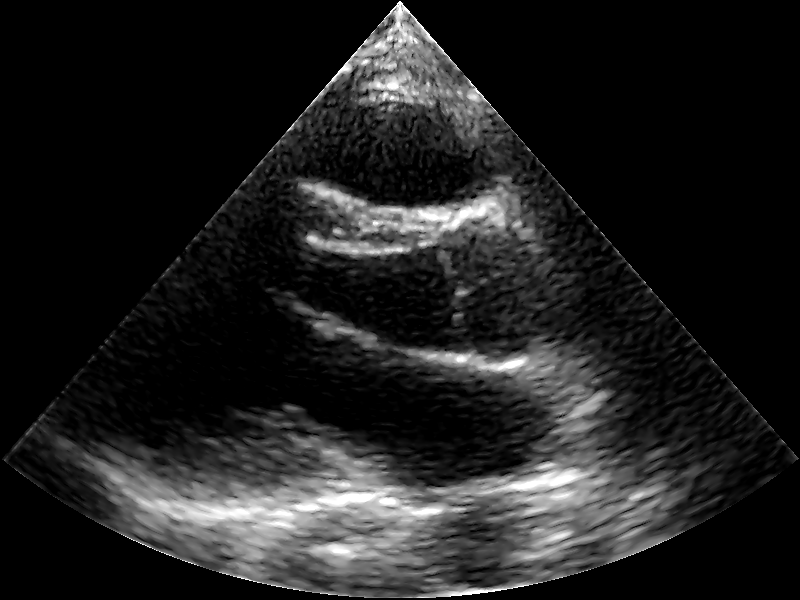
\includegraphics[width=\textwidth]{figures/cardiac1_clpdb.png}};
      \spy on (0.05, 0.05) in node [redwindow, anchor=north] at ($(figA.south)$);
    \end{tikzpicture}
    \caption{CLPD-B}
  \end{subfigure}%
  \begin{subfigure}[b]{0.15\textwidth}
    \begin{tikzpicture}[
        spy using outlines={%
          rectangle,magnification=3,size=\textwidth,
          every spy on node/.append style={transparentwindow}
        }
      ]
      \node (figA) at (0.0,0.0) {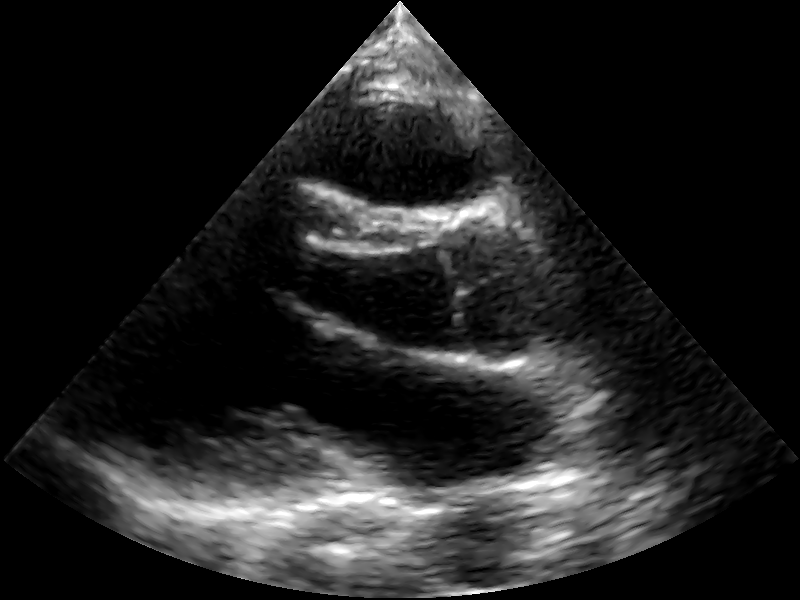
\includegraphics[width=\textwidth]{figures/cardiac1_clpdc.png}};
      \spy on (0.05, 0.05) in node [redwindow, anchor=north] at ($(figA.south)$);
    \end{tikzpicture}
    \caption{CLPD-C}
  \end{subfigure}%
  \begin{subfigure}[b]{0.15\textwidth}
    \begin{tikzpicture}[
        spy using outlines={%
          rectangle,magnification=3,size=\textwidth,
          every spy on node/.append style={transparentwindow}
        }
      ]
      \node (figA) at (0.0,0.0) {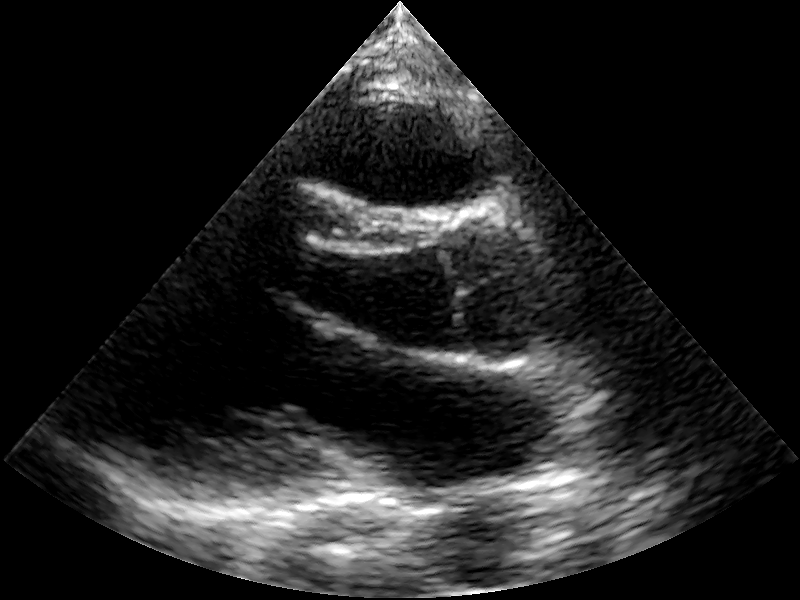
\includegraphics[width=\textwidth]{figures/cardiac1_clpdd.png}};
      \spy on (0.05, 0.05) in node [redwindow, anchor=north] at ($(figA.south)$);
    \end{tikzpicture}
    \caption{CLPD-D}
  \end{subfigure}%
  \begin{subfigure}[b]{0.15\textwidth}
    \begin{tikzpicture}[
        spy using outlines={%
          rectangle,magnification=3,size=\textwidth,
          every spy on node/.append style={redwindow}
        }
      ]
      \node (figA) at (0.0,0.0) {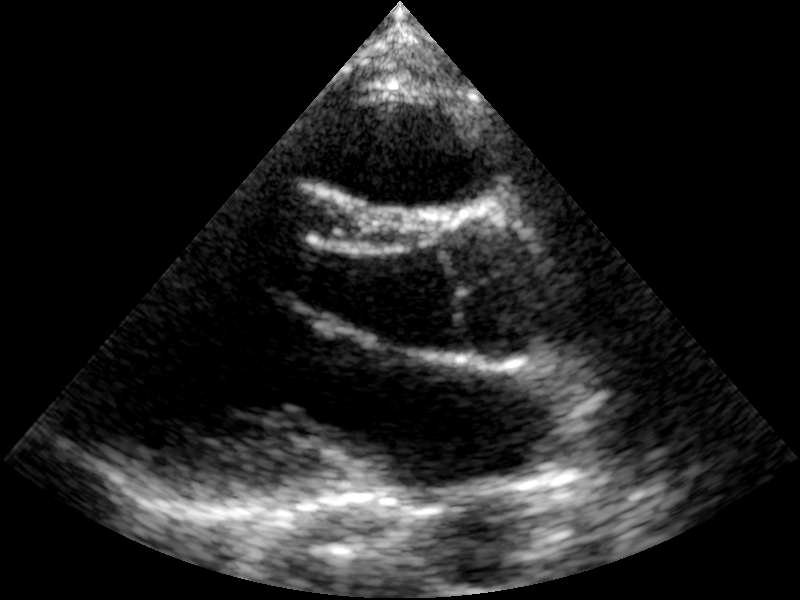
\includegraphics[width=\textwidth]{figures/cardiac1.png}};
      \spy on (0.05, 0.05) in node [redwindow, anchor=north] at ($(figA.south)$);
    \end{tikzpicture}
    \caption{Original}
  \end{subfigure}
  \caption{Results on echocardiography parasternal long-axis view.}\label{fig:cardiac1}
  \vspace{-0.1in}
\end{figure*}

%%% Local Variables:
%%% TeX-master: "master"
%%% End:

%
\subsection{Results on Echocardiographic 4-Chamber View}
We now present results on a sequence of echocardiographic 4-chamber view images.

\subsubsection{Qualititative Results}
A single frame from each processed result is shown in~\cref{fig:cardiac3}.

Similarly with the liver image, CLPD-A to CLPD-F turned out to be the least blurry.
Unlike the liver image, however, some of the expert tuned CLPDs showed strong speckle reduction.
For example, CLPD-F shows the cleanest myocardium wall among all methods.
Despite the strong smoothing effect, it does not result in blurry images such as NLLR, which shows the effectiveness of the cascaded Laplacian pyramid approach.

In addition, CLPDs resulted in smooth myocardium edges, thanks to the multiscale analysis of the Laplacian pyramid.
In contrast, other methods result in jiggly myocardium edges due to structural dagmaes caused by speckle.
While NLLR results in the best structural enhancement, the resulting blurriness shadows its benefits.

Meanwhile, CLPD-A results in amplified fine details.
Indeed, the cardiologist (A) who tuned CLPD-A expressed his preference for fine details such as papillary muscles.
This shows the preferential difference between cardiologist and sonographers.
Overall, the results on the echocardiographic 4-chamber view show that image enhancement methods need to be tuned, not only to each individual, but also each clinical task.

\subsubsection{Quantitative Results}
We now discuss the quantitative results on the echocardiographic 4-chamber image.

For the echocardiographic images, correctly recognizing different anatomical structures and thier borders is clinically important.
Therefore, unlike the liver image, speckle reduction and contrast enhancement is more relevant.
This is clearly reflected in~\cref{table:cardiac3}.
All CLPD settings showed the highest SNR on the myocardium wall.
In terms of contrast, sonographer B and F showed preference towards high gCNR and CNR.
However, CLPDs still achieved high SSIM and \(S_3\).

Among the considered baselines, MNLM and NLLR achieved the highers contrast.
Still, both methods are known to be good at removing speckle.
However, they both resulted in low sharpness, where NLLR resulted in an unbelievely low \(S_3\) value.
Meanwhile, except for NLLR, all methods did not achieve a high SNR.
Although this is expected with ADMSS since it deliberately avoids reducing speckle on structural regions, the low SNR of MNLM is counter-intuitive.
From visual inspection, this seems to be a result of MNLM and other methods not improving the homogeneity of similar anatomical regions.
NLLR and CLPDs, on ther other hand, improve the structural homogeneity.
This shows the importance of structural enhancement for echocardiographic images, which CLPDs achieve by coherence enhancement in higher scales.

\subsection{Results on Echocardocraphic Parasternal Long-Axis View}
Finally, we present qualitative results on an echocardocraphic parasternal long-axis view sequence.
The parasternal long-axis view has many clinically relevant fine details such as the mitral valve and the aortic valve.
These fine details, however, are difficult to differentiate from speckle and clutter.

The results are shown in~\cref{fig:cardiac3}.
Unlike the echocardiographic 4-chamber view, all CLPDs amplify fine-details regardless of speckle and clutter.
Flow-like artifacts resulting from aggressive coherence enhancement are clearly visible near the aortic valve.
As a result, the edges of the interventricular septum are enhanced.

%%% Local Variables:
%%% TeX-master: "master"
%%% End:
